\thispagestyle{fancy}
\justifying
\section{Untersuchung optisch gepumpter Laserstrukturen auf unterschiedlichen Templates}
Dieses Kapitel widmet sich der Untersuchung zweier Probenreihen von optisch gepumpten Laserstrukturen, die aus Rezepten aus zwei unterschiedlichen Serien stammen. Die beiden Serien unterscheiden sich im wesentlichen dadurch, dass sie mit(Serie 2) und ohne Übergitter(Serie 1)gewachsen wurden. Sie haben alle eine aktive Zone, die sich zusammen setzt aus zwei $5$nm dicken und siliziumdotierten $ Al_{0.8}Ga_{0.3}N$-Barrieren zwischen den drei $2.2$nm dicken $ Al_{0.56}Ga_{0.44}N$ QWs. Die aktive Zonne befindet sich zwischen einem $30 \thinspace nm$ dicken $ Al_{0.70}Ga_{0.30}N$ und einem $85 \thinspace nm$ dicken Waveguide als oberste Schicht. Der Wellenleiter hat den Zweck, die optische Mode einzuschließen, daher ist ein hoher Brechungsindexsprung zwischen den Barrieren der aktiven Region und der darüberlegenden Schichten notwendig.
Dieser Block an Schichten bildet die unveränderte Grundlage für alle in diesem Kapitel untersuchten Proben.
Die Proben weisen untereinander Unterschiede in ihren Substraten auf, so sind zwei Proben der Serie 1 auf AlN-Bulk zweier unterschiedlicher Hersteller (HexaTech, IKZ) gewachsen und alle anderen Proben auf ELO AlN/Sapphire mit jeweils 3 unterschiedlichen  Fehlschnitt-Winkeln. Tabellarisch sieht die Zusammenstellung wie folgt aus: 
\begin{figure}[H]
\centering
\begin{tabular}{ |c|c|c|c|c|c|   }
\hline
\multicolumn{3}{|c|}{Serie 1} & \multicolumn{3}{c|}{Serie 2}  \\
\hline
Name & offcut& Template & Name& offcut & Template \\
\hline
A & 0.1$^\circ$m & ELO & A-SL & 0.1$^\circ$m & ELO \\
B & 0.1$^\circ$m* & ELO & B-SL & 0.1$^\circ$m* & ELO \\
C & 0.2$^\circ$m & ELO & C-SL & 0.2$^\circ$m & ELO \\
D & 0.1$^\circ$m & Bulk(IKZ) &  & &  \\
E & 0.1$^\circ$m & Bulk(Hexatech) & & & \\
\hline
\end{tabular}
\end{figure}
\noindent 
Die Proben beider Serien mit dem ELO AlN/Saphir Substrat unterscheiden sich untereinander noch vom Fehlschnitt und der Richtung des Fehlschnittes des Substrats. Die gegeben Werte stammen vom Hersteller und sind nur nominelle Werte die sich von den realen unterscheiden können. So haben die mit A gekennzeichneten Proben einen nominellen Fehlschnitt von $\alpha = 0.1\circ \thinspace m$ in die Standard m-Richtung, die mit B gekennzeichneten Proben den selben Fehlschnitt in eine der sechs nicht Standard m-Richtungen und die mit C gekennzeichneten Proben einen Fehlschnitt von $\alpha = 0.2\circ \thinspace m$ in die Standard m-Richtung. 
Die Untersuchung des Einflusses des Fehlschnitt-Winkels des Substrates, ist insofern interessant, da dieser eine entscheidende Rolle beim Wachstum der Heterostrukturen spielt. Er erlaubt es die Wachstumskinetik zu steuern, so dass sich die Schichten in die kristalline Struktur  formen wie in Abbildung \ref{fig:offcut} zu sehen ist.
Der Fehlschnitt-Winkel $\alpha$ ist die Winkel-Differenz zwischen Oberflächennormale und der c-Richtung. Für ein $\alpha \leq 0,12 $ wurde gezeigt, dass es zu Stufenfluss kommt und somit zu relativ glatten Oberflächen mit wellenartiger Morphologie und mit $\alpha \geq 0,16 $ in Stufenbündelwachstum mit Makrostufen resultieren kann. Dies ist nicht unwichtig für Laserstrukturen, da glatte Oberflächen optische Streuung an der Oberfläche verringern, sollten aber keinen Effekt auf die IQE haben. Allerdings kann an den Stufenkanten verstärkt Ga eingebaut und somit die Zusammensetzung der aktiven Zone inhomogen werden \cite{zeimeru} \cite{MOGILATENKO2014222} \cite{fmehnke}, was wiederum einen Einfluss auf die IQE durch Lokalisierung haben könnte.
%
\begin{figure}[htb]
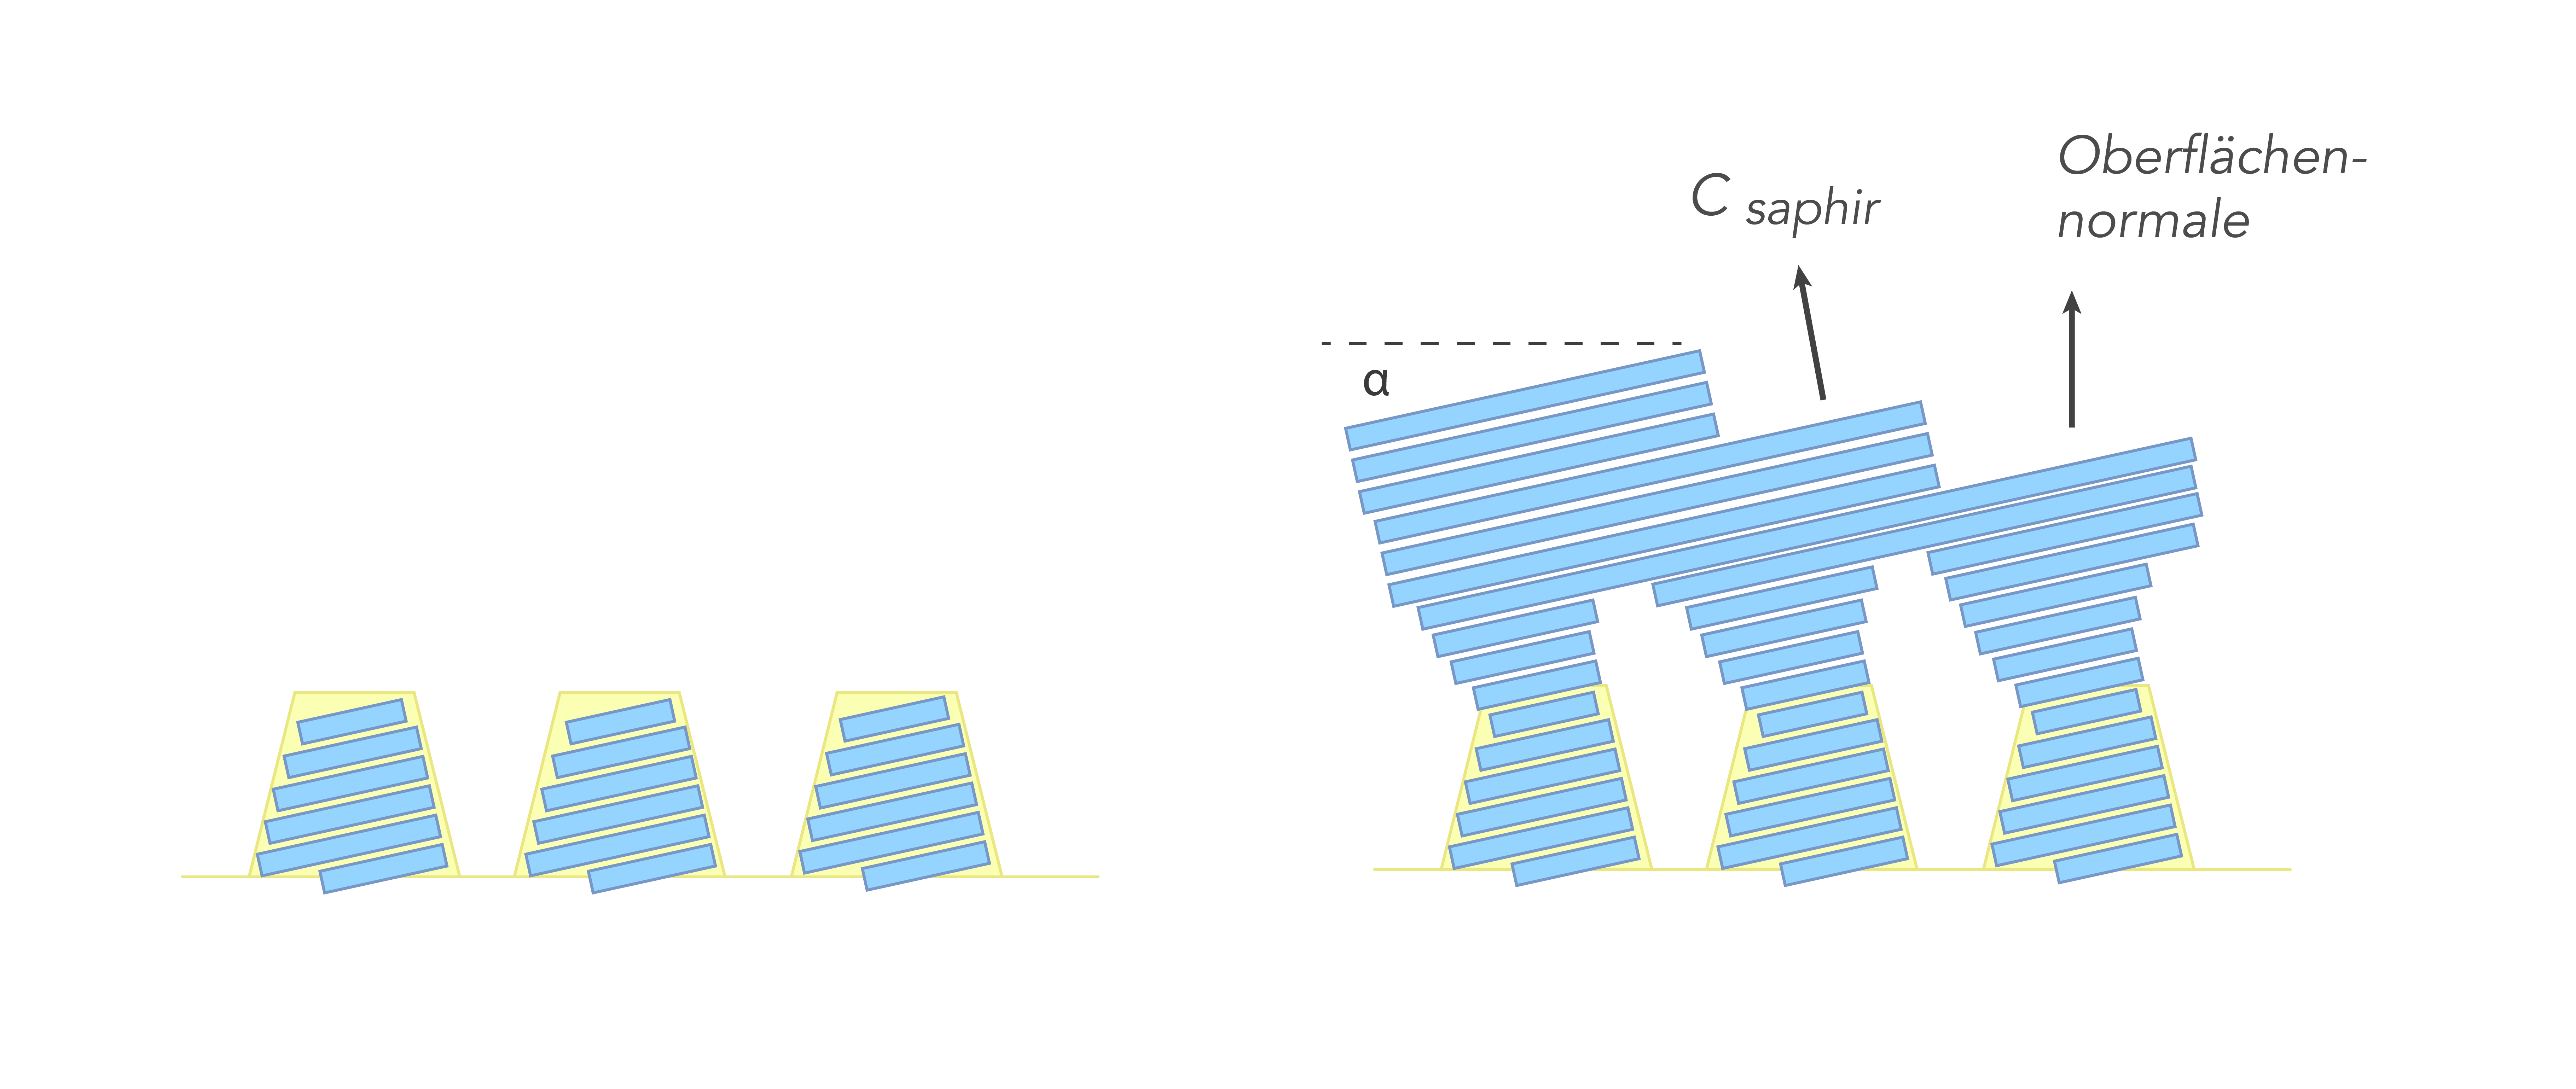
\includegraphics[width=\linewidth]{Bilder/offcut.png}
\caption{Einfluss des Fehlschnitt-Winkels auf das Wachstum bei ELO AlN/Saphir.}
\label{fig:offcut}
\end{figure}
\noindent 
\vspace{1cm}
%
Die Makrostufen können zudem zu einer Reduktion der TDD beitragen, die wiederum in der IQE sichtbar ist wie Abb. [\ref{fig:IQEthreadingdisl}] zeigt. Bei Proben mit einem geringen Fehlschnitt von $\alpha = 0,12 $ verlaufen die Versetzungen senkrecht zur Kristalloberfläche. Bei Proben mit einem großen Fehlschnitt von $\alpha = 0,16 $ verlaufen die Versetzungen diagonal wie Abb. [\ref{fig:schraubenvers}] zeigt. Bei diesen Versetzungen handelt es sich um sogenannten Koaleszenzkorngrenzen die an der Oberfläche als Makrostufen zu erkennen sind \cite{MOGILATENKO2014222}. 
%
\begin{figure}[htb]
  \centering
  \begin{minipage}[t]{0.49\textwidth}
    \centering
    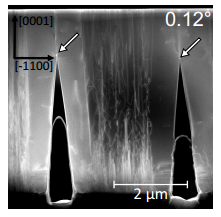
\includegraphics[width=0.6\textwidth]{Bilder/offcutsenkrecht.png}
    \label{}
  \end{minipage}
	\hfill
  \begin{minipage}[t]{0.49\textwidth}
    \centering
    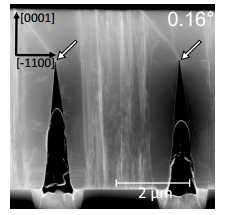
\includegraphics[width=0.6\linewidth]{Bilder/offcutdiagonal.png}
    \label{}
  \end{minipage}
	\caption{Querschnitts-TEM-Aufnahmen mit den sichtbaren senkrecht und diagonal verlaufenden Schraubenversetzungen}
	\label{schraubenvers}
\end{figure}
%
Bei Schichtdicken $ \geq 10 \mu m $ kreuzen diese diagonal verlaufenden Makrostufen die versetzungsreichen Gebiete zwischen den geätzten Gräben im ELO oft genug um diese fast vollständig zu annhilieren \cite{fmehnke}. Solche Dicken sind aber schwierig zu realisieren durch das schwierige Wachstum und der entstehenden Krümmung des Wafers. Bei den hier verwendeten Schichtdicken von $ \geq 1 \thinspace \mu m $ ist nur eine teilweise Annihilation und damit eine Defektreduktion von $1\cdot 10^{10} \thinspace cm^{-2}$ auf $5\cdot 10^9 \thinspace cm^{-2}$ zu erwarten \cite{fmehnke}. Weiter beachtet werden muss, dass bei den darauf folgenden Schichten eine Planarisierung stattfinden muss, um eine möglichst ebene aktive Zone zu haben. 
\newpage
\subsection{UVC-Laser Strukturen auf ELO ohne Übergitter}
%
\begin{figure}[h]
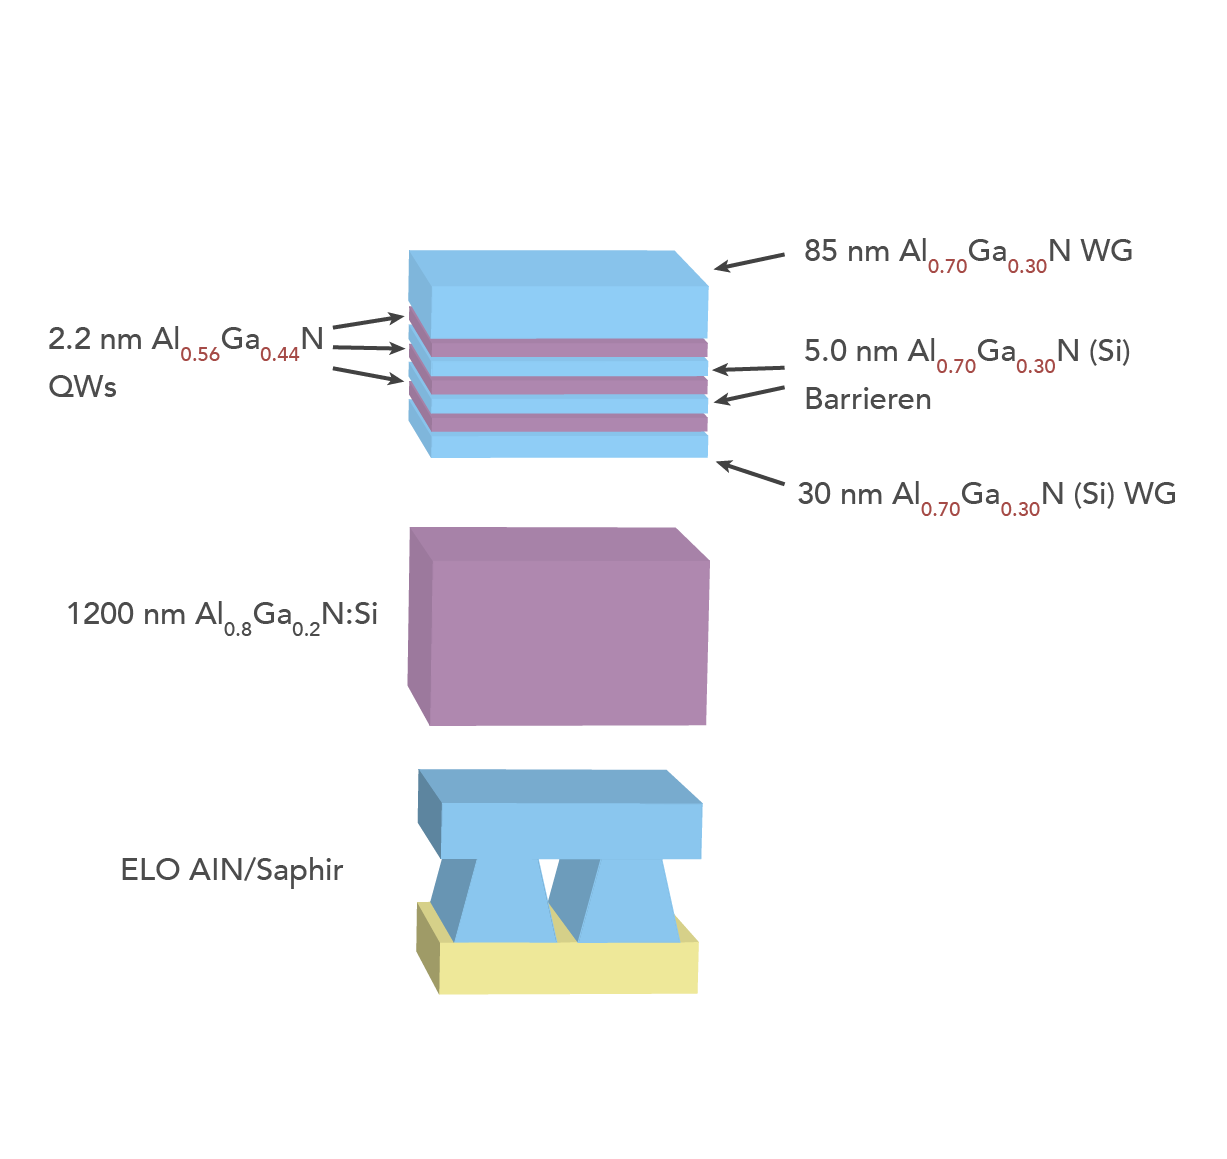
\includegraphics[width=\linewidth]{Bilder/TS4045/ts4045.png}
\caption{Schichtstruktur der untersuchten Proben.}
\label{fig:schichtenelo}
\end{figure}
\noindent 
\vspace{1cm}
%
Die drei untersuchten Proben A-ELO, B-ELO und C-ELO setzen sich zusammen aus der oben genannten aktiven Zone. Das Substrat ist ELO AlN/Saphir und darauf aufgewachsen wurde eine $1200 \thinspace nm$ dicke $ Al_{0.8}Ga_{0.2}N$-Bufferschicht (Abb. [\ref{fig:schichtenelo}]). Die zentrale Wellenlänge der Proben befindet sich bei $(271 \pm 1) \thinspace nm$ wie in Abb. [\ref{fig:spectraselo}] zu sehen ist. Durch die nicht resonante Anregung ist der QW-Peak und auch der QB-Peak bei Tieftemperatur bei allen Proben zu sehen, der Anteil des QB-Peaks sinkt aber mit steigender Temperatur durch die steigende kinetische Energie der Elektronen, die bevorzugt in die Leitungsbandminima (den QWs) wandern (thermisches Diffundieren).
%
\begin{figure}[htb]
  \centering
  \begin{minipage}[t]{0.4\textwidth}
    \centering
    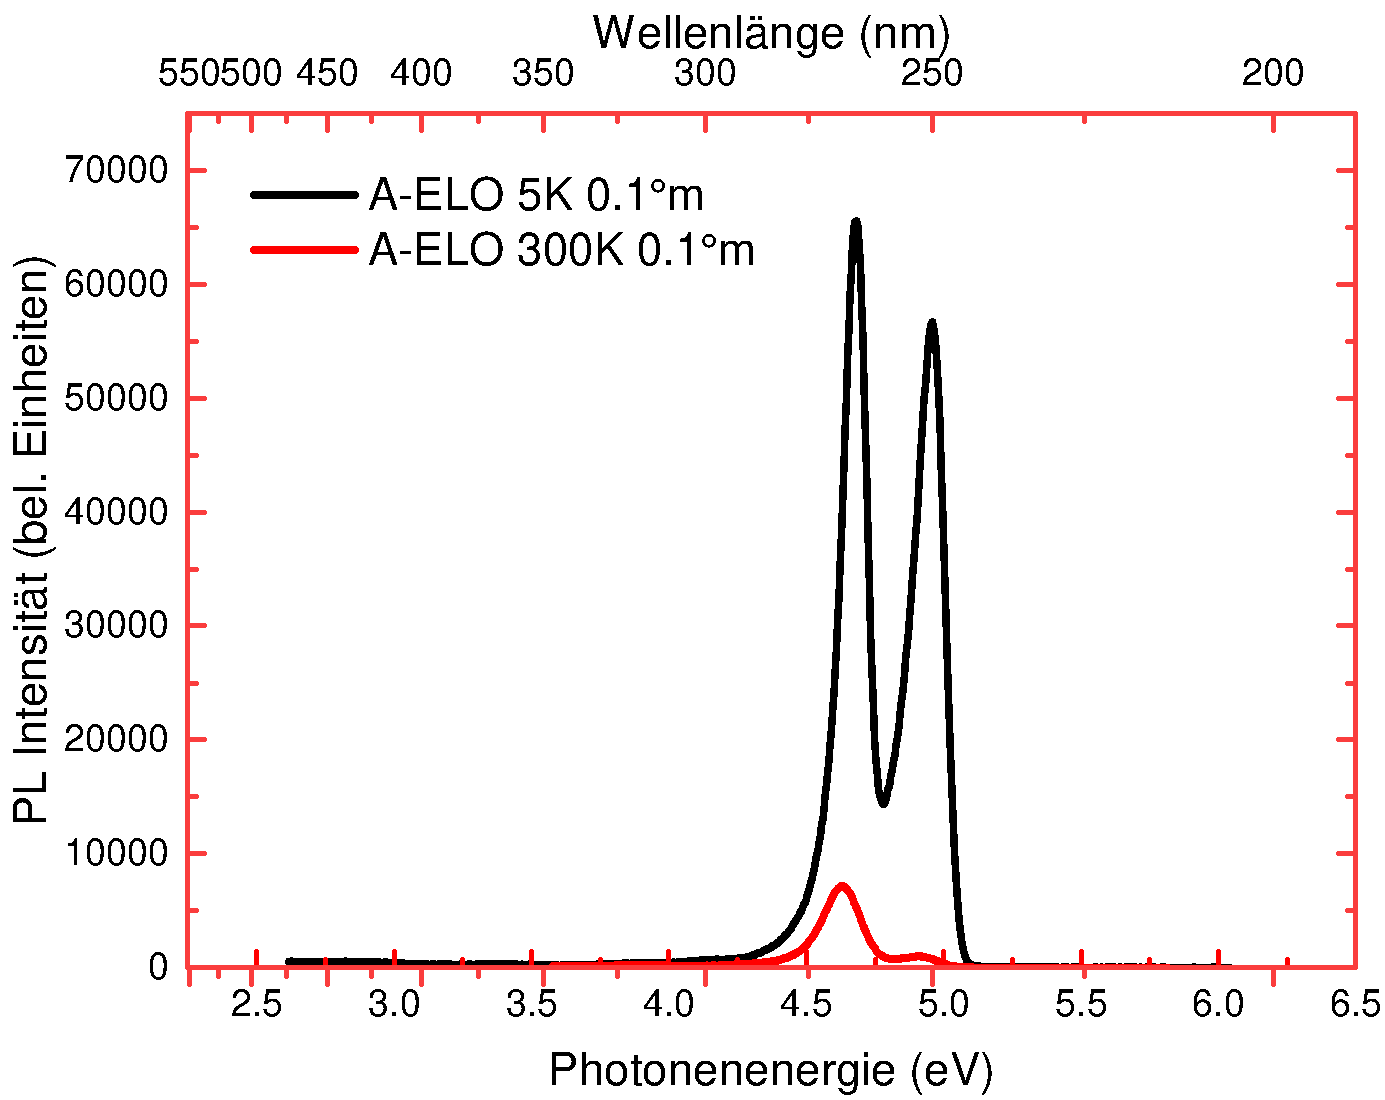
\includegraphics[width=\textwidth]{Bilder/TS4045/aelo.pdf}
  \end{minipage}
	\hfill
  \begin{minipage}[t]{0.4\textwidth}
    \centering
    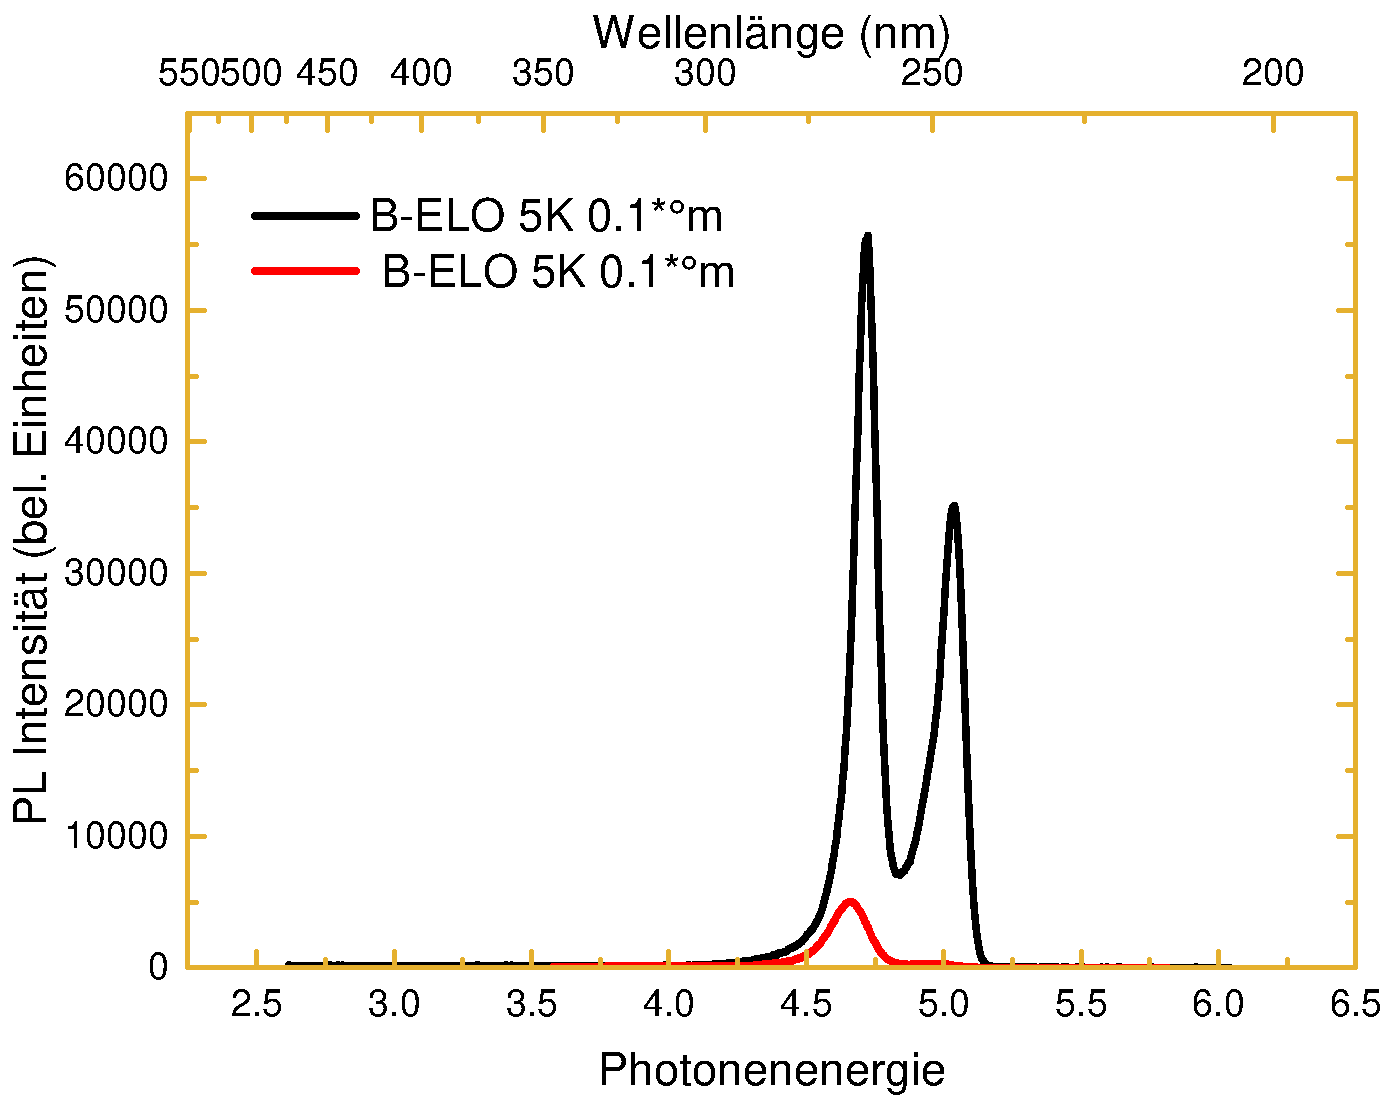
\includegraphics[width=\linewidth]{Bilder/TS4045/belo.pdf}
  \end{minipage}
	\hfill
  \begin{minipage}[t]{0.4\textwidth}
    \centering
    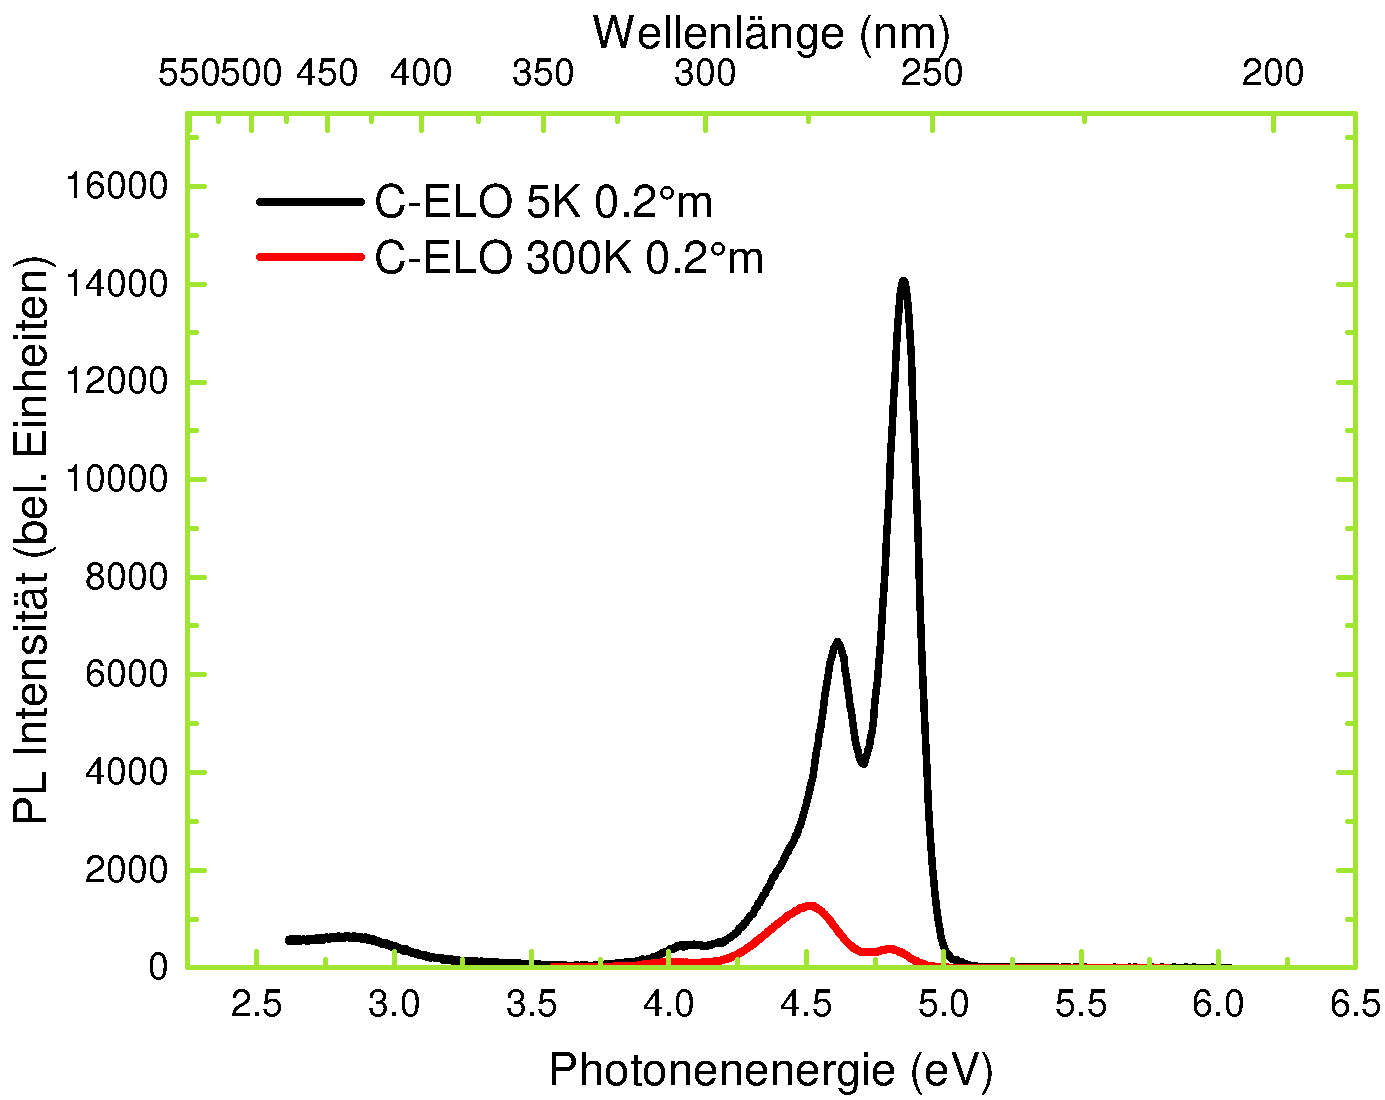
\includegraphics[width=\linewidth]{Bilder/TS4045/celo.pdf}
  \end{minipage}
	\caption{Aufnahme der Spektren der Proben A-ELO mit einem Fehlschnittwinkel von $0.1$ in die Standard m-Richtung, Probe B-ELO mit einem Fehlschnittwinkel von $0.1$ die andere m-Richtung und Probe C-ELO mit einem Fehlschnittwinkel von $0.2$ in die standard m-Richtung. }
	\label{fig:spectraselo}
\end{figure}
\noindent 
%
Die Probe C-ELO zeigt bei TT ein abweichendes Verhalten bezüglich der Verteilung der Intensität auf QB-Peak und QW-Peak. Ein möglicher Grund könnte die Fokussierung sein oder der oberste Waveguide der den gleichen Al-Gehalt hat wie die QBs, absorbiert einen Großteil des Lichtes bevor es in die QWs gelangt. 
Anhand der Intensitäten allein, ist noch kein Rückschluss auf die IQE der Proben zu schliessen., bedingt durch die unterschiedliche Positionierung der Proben und der Fokussierung. Dennoch ist hier bereits auffällig, dass die Probe C-ELO (grün) eine deutlich geringere Intensität bei RT und TT hat.
%
\begin{figure}[htb]
  \centering
  \begin{minipage}[t]{0.49\textwidth}
    \centering
    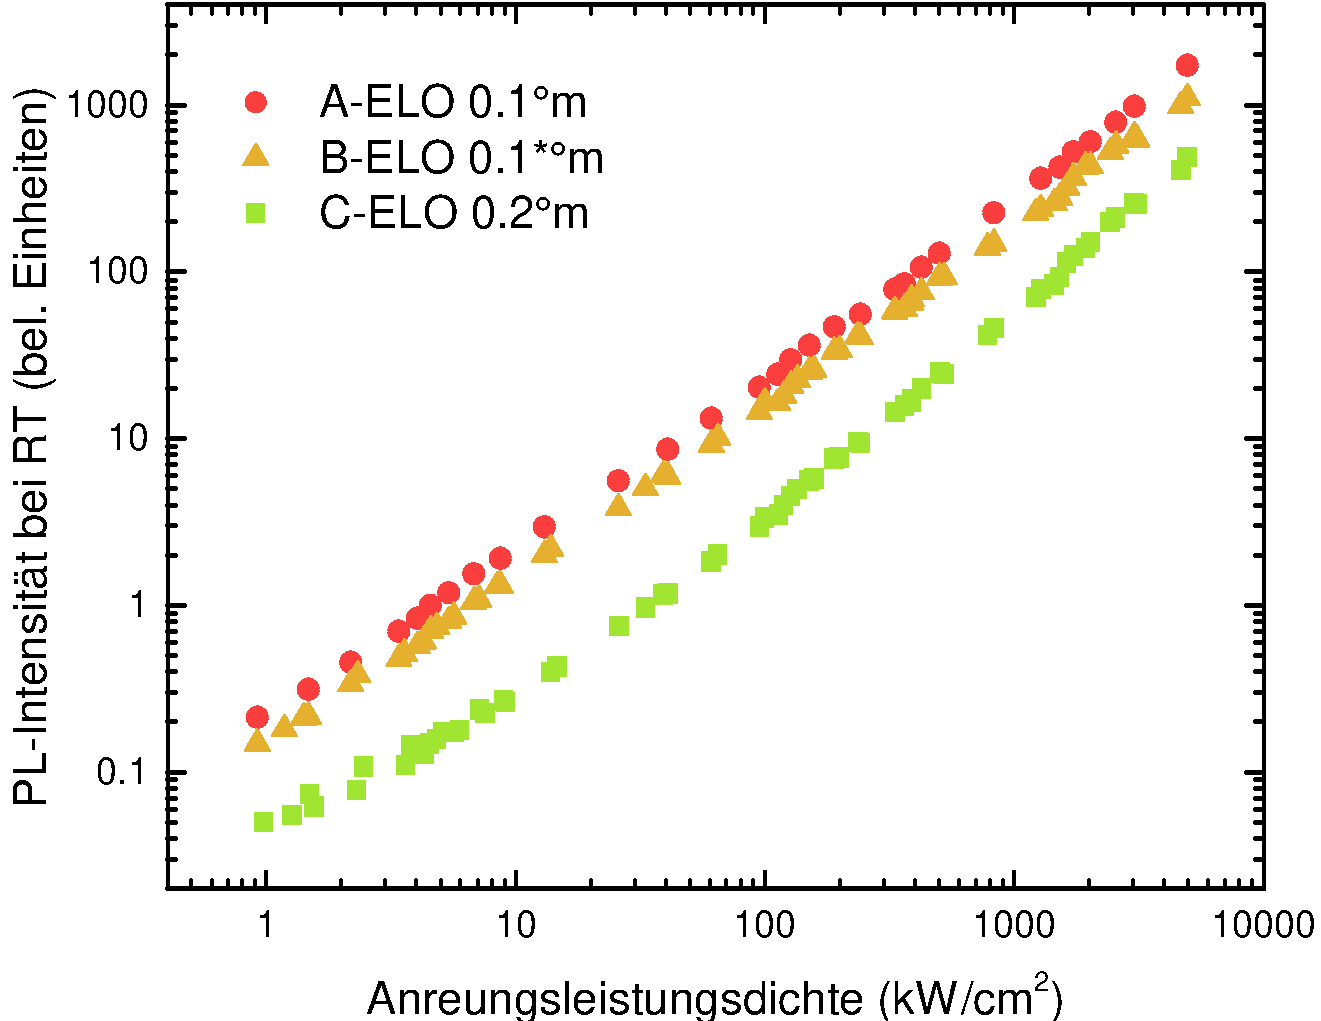
\includegraphics[width=\textwidth]{Bilder/TS4045/intRT.pdf}
		\caption{}
    \label{fig:eloINTrt}
  \end{minipage}
	\hfill
  \begin{minipage}[t]{0.49\textwidth}
    \centering
    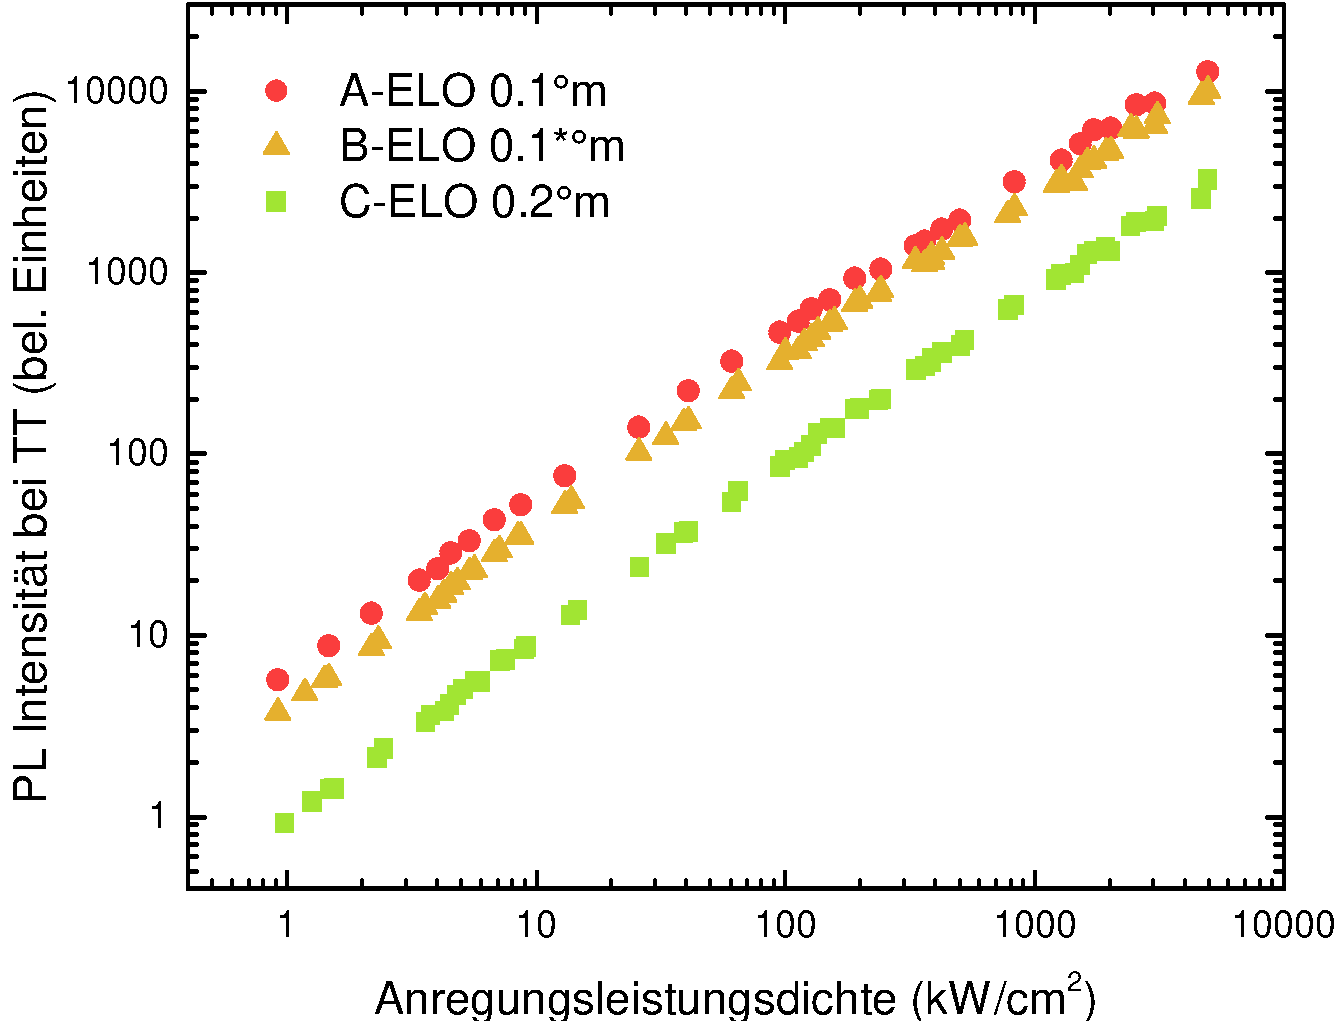
\includegraphics[width=\linewidth]{Bilder/TS4045/intTT.pdf}
    \label{fig:eloINTtt}
		\caption{}
  \end{minipage}
	\caption{Die integrierte Intensität in Abhängigkeit der Anregungsleistungsdichte bei Raum- und Tieftemperatur in doppelt-logarithmischer Darstellung. }
\end{figure}
\noindent 
% 
Dies bestätigt sich in den Abbildungen [\ref{fig:eloINTrt}] und [\ref{fig:eloINTtt}]. Die Proben A-ELO und B-ELO zeigen keinen signifikanten Unterschied in den Intensitäten zueinander, der Rückschlüsse auf unterschiedliche IQEs erlauben würde.  Bei der Probe C-ELO kann also durch den drastischen Unterschied direkt anhand der Spektren gesagt werden, dass sie die geringste IQE haben müsste, da sie mit deutlichem Abstand am schwächsten leuchtet obwohl bei allen Proben die gleiche Fläche beleuchtet wird. Letzteres bedeutet, dass eigentlich die gleiche Anzahl an Ladungsträgern in den Proben generiert werden sollte und so ein erheblicher Unterschied in den Intensitäten nur durch eine deutliche höhere nicht-radiative Rekombination in der Probe C-ELO zu erklären ist.
%
\begin{figure}[H]
  \centering
  \begin{minipage}[t]{0.49\textwidth}
    \centering
    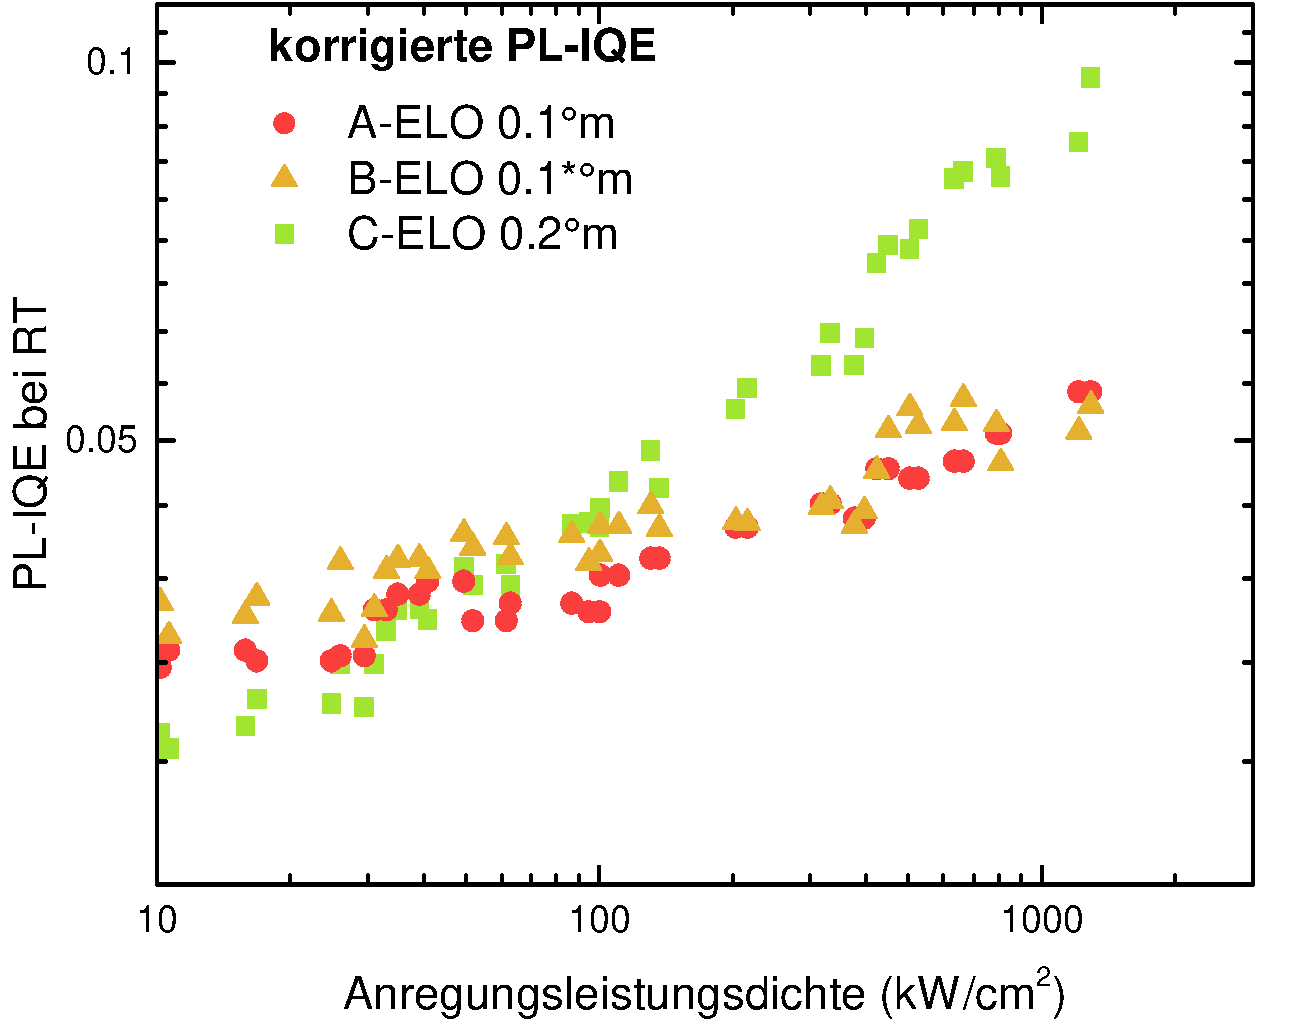
\includegraphics[width=\textwidth]{Bilder/TS4045/corrIQERT.pdf}
    \label{fig:eloiqeRT}
  \end{minipage}
	\hfill
  \begin{minipage}[t]{0.49\textwidth}
    \centering
    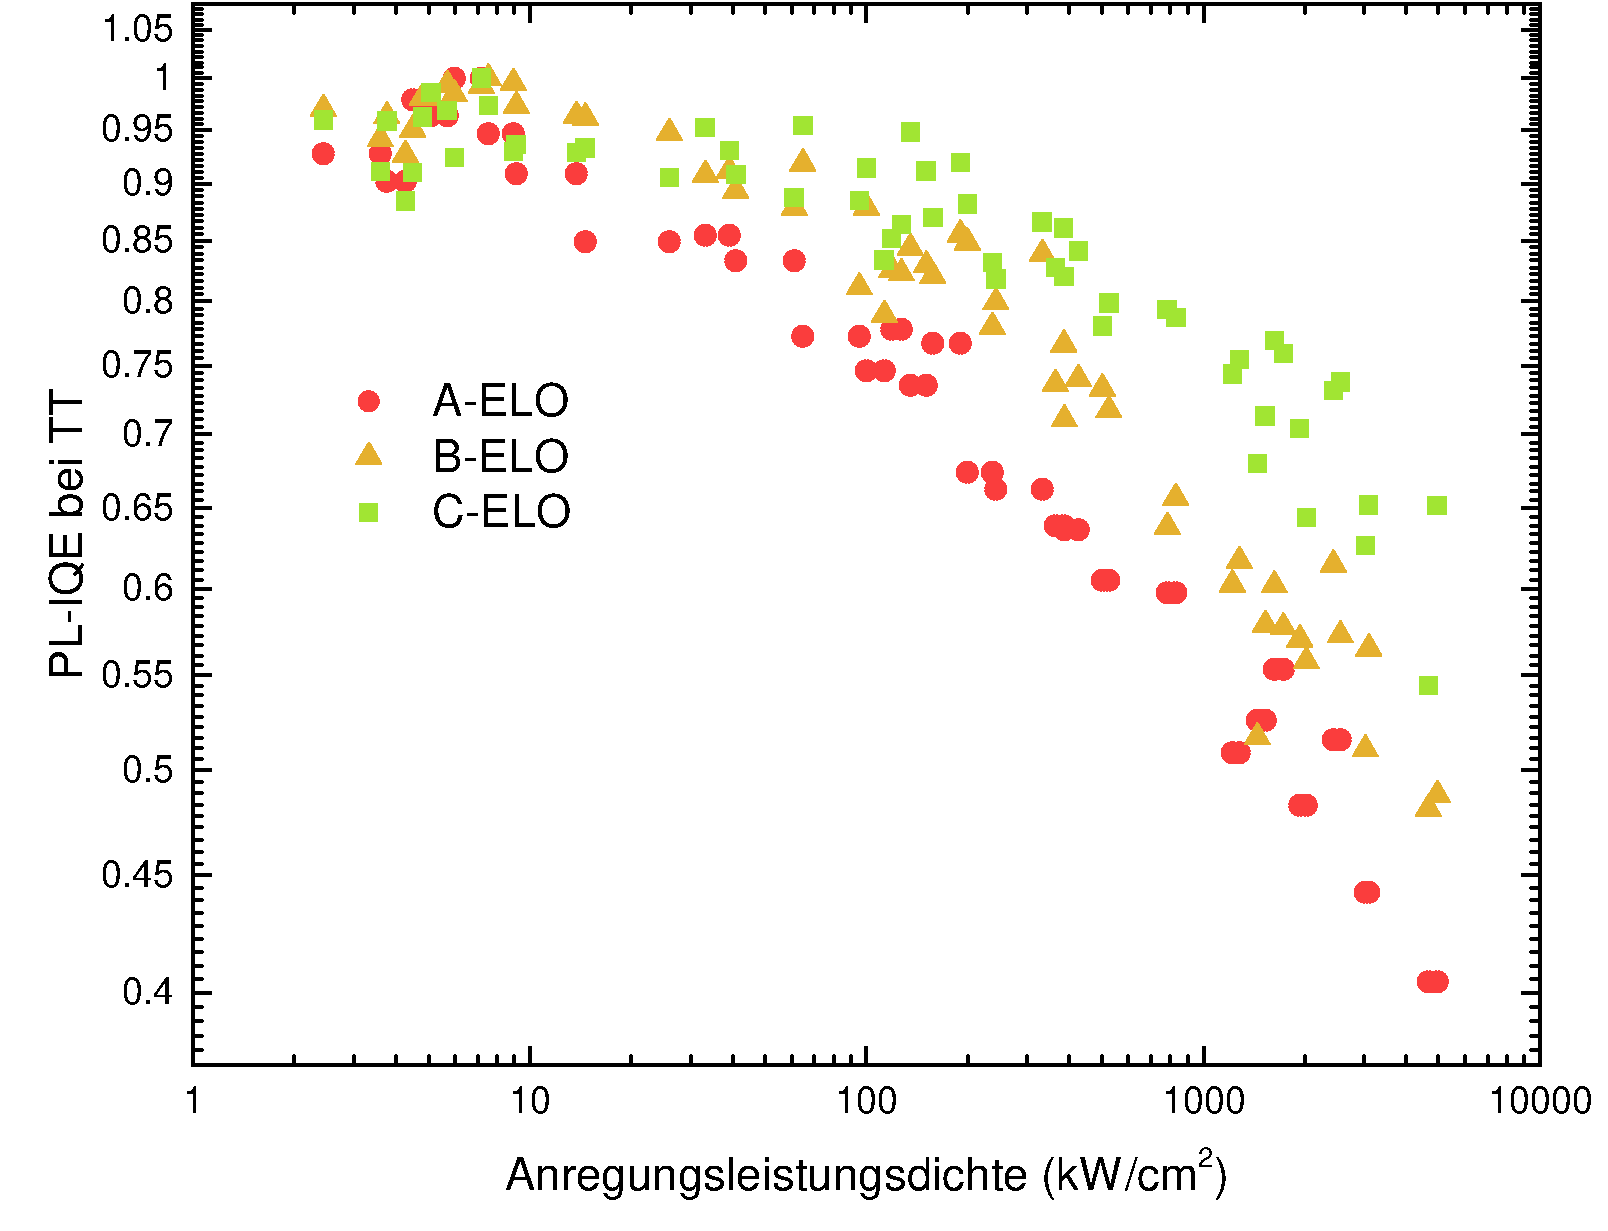
\includegraphics[width=\linewidth]{Bilder/TS4045/IQETT.pdf}
    \label{fig:elocorriqeRT}
  \end{minipage}
	\caption{Die IQEs für die Proben A-ELO, B-ELO und C-ELO bei Raumtemperatur und Tieftemperatur.}
\end{figure}
\noindent 
%
Die Ergebnisse für die IQE bei RT zeigen allerdings etwas anderes, wie in Abbildung [\ref{fig:eloiqeRT}] zu sehen ist. 
So ist die IQE bei der Probe C-ELO mit einem Wert von $IQE_{C-ELO} = 0,0028$
im Bereich von geringen Anregungsleistungsdichten von $ 10 \frac{kW}{cm^2} $ bis $ 100 \frac{kW}{cm^2} $ niedriger als für die Proben A-ELO und B-ELO, die sich, wie aus den Intensitäten und ihren Verhältnissen bei TT und RT bereits zu vermuten ist, ähnlich verhalten. 
Die IQE für die Probe C-ELO weist indes eine deutlich stärkere Steigung auf, sodass die IQE mit zunehmender Anregungsleistungsdichte die der Proben A-ELO und B-ELO immer deutlicher übersteigt. Sodass bei der höchsten Anregungsleistungsdichte $ 1300 \frac{kW}{cm^2} $ die IQE der Probe C-ELO mit einer IQE von $IQE_{C-ELO} = 0,0098$ (9,8 \%) die der Proben A-ELO mit $IQE_{A-ELO} = 0,0055$ (5,5 \%) und B-ELO mit $IQE_{B-ELO} = 0,0054$ (5,4 \%) um fast das doppelte übersteigt. Werden zusätzlich die IQEs bei $5K$ berachtet, ist ersichtlich, dass die IQEs Proben A-ELO und B-ELO erheblich schneller absinken als die der Probe C-ELO. Dieser erreicht mit sinkender Anregungsleistungsdichte das Plataeu , dass bei geringen Anregungsleistungen aufgrund der $n^3$ Abhängigkeit der Auger-Rekombination zu erwarten ist. A-ELO und C-ELO dagegen scheinen dieses Plataeu nicht zu erreichen. Daraus resultierend, liegt die Schlussfolgerung nahe, dass die hier verwendeten Anregungsleistungsdichten für die Proben A-ELO und B-ELO nicht gering genug und somit die IQEs unterbewertet sind, zudem ist das unterschiedliche Verhalten der IQEs bei $5K$ möglicherweise dadurch zu erklären, dass auf die Probe C-ELO nicht die gleiche Anzahl an Ladungsträgern die aktive Zone erreichen. Was im Umkehrschluss erklärt, wieso das Plataeu bei der Probe C-ELO früher erreicht wird, da somit die tatsächlich auf der Probe ankommende Anregungsleistungsdichte geringer ausfällt.  
%
\begin{figure}[H]
\begin{tabular}{ccc}
  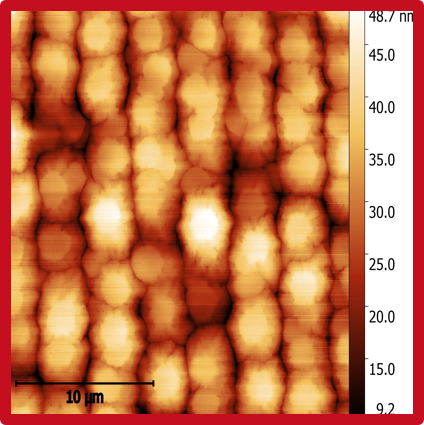
\includegraphics[width=0.35\textwidth]{Bilder/TS4045/aELOafm.png} & 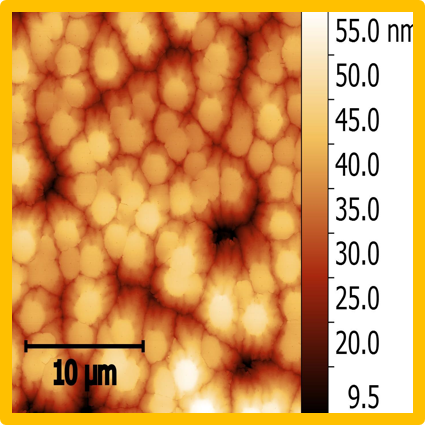
\includegraphics[width=0.35\textwidth]{Bilder/TS4045/bELOafm.png}  & 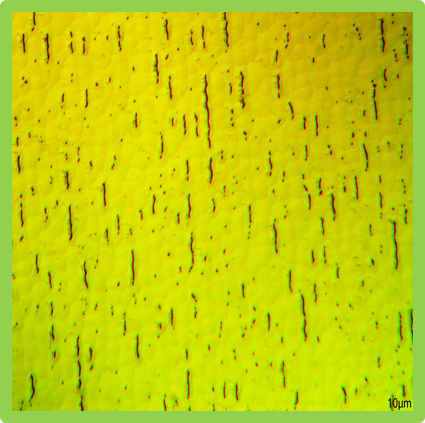
\includegraphics[width=0.35\textwidth]{Bilder/TS4045/cELOlimi.png} \\
(a) & (b) & (c) \\[6pt]
 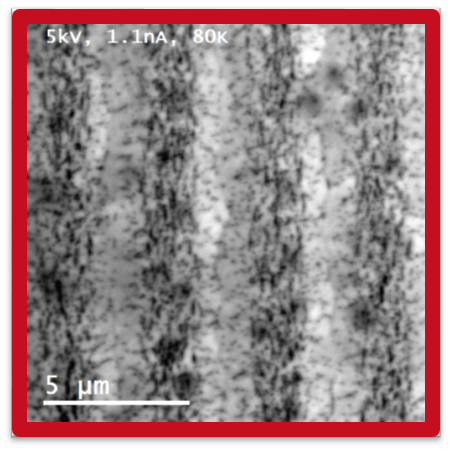
\includegraphics[width=0.35\textwidth]{Bilder/TS4045/aELOcl2.png} &   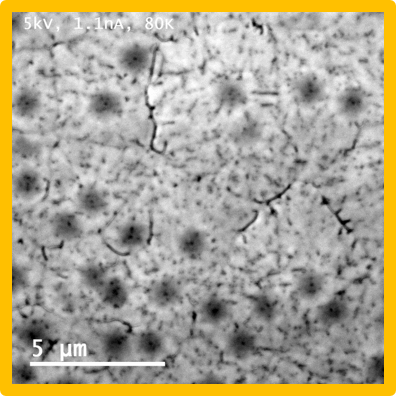
\includegraphics[width=0.35\textwidth]{Bilder/TS4045/bELOcl2.png} & 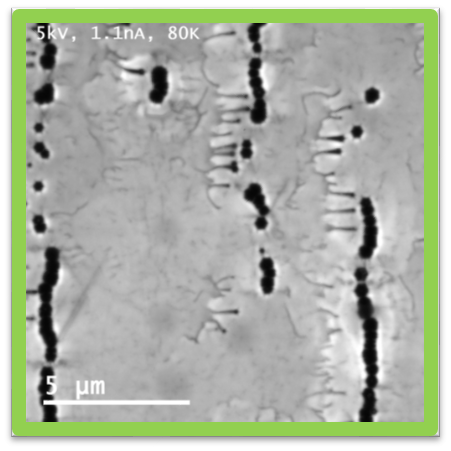
\includegraphics[width=0.35\textwidth]{Bilder/TS4045/cELOcl2.png}  \\
(c)  & (d) & (e)   \\[6pt]
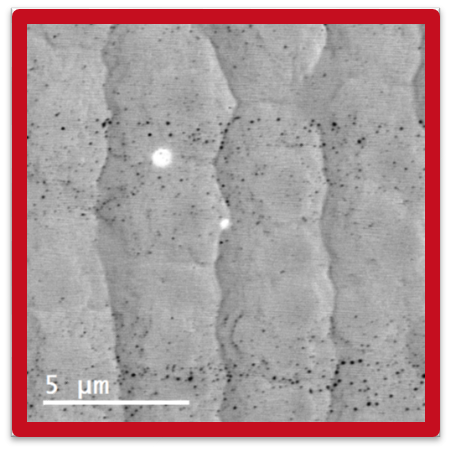
\includegraphics[width=0.35\textwidth]{Bilder/TS4045/aELOcl1.png} & 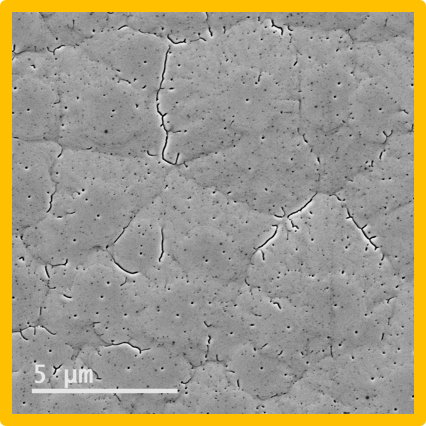
\includegraphics[width=0.35\textwidth]{Bilder/TS4045/bELOcl1.png}  & 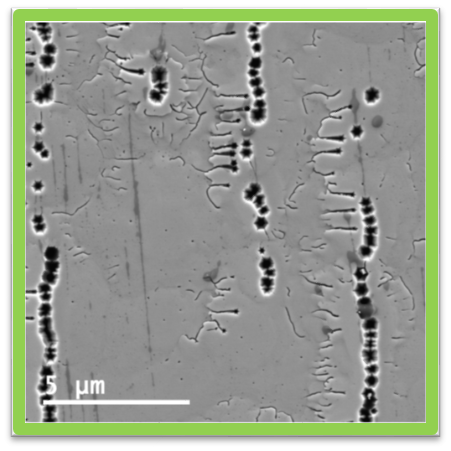
\includegraphics[width=0.35\textwidth]{Bilder/TS4045/cELOcl1.png} \\
(f)  & (g) & (h)   \\[6pt]
\end{tabular}
\caption{AFM-Bilder (a, b) und eine Limi-Aufnahme (c) von Christian Kuhn aufgenommen. SEM (c, d, e) und panchromatische CL-Aufnahmen(f, g, h) an den selben Stellen gemessen von Ute Zeimer (FBH)}
\label{fig:morph1}
\end{figure}
\noindent 
Um die Gründe für diese Unterschiede in den IQEs und den Einfluss des Fehlschnittes auf die Oberflächenmorphologie weiter zu untersuchen, werden AFM-Aufnahmen und panchromatische CL-Aufnahmen und dazu von derselben Stelle Rasterelektronenmikroskopie-Aufnahmen betrachtet und auf ihre Besonderheiten analysiert. Die CL-Bilder wurden bei einer Beschleunigungsspannung von 5 kV,
einer Stromstärke von 1,1 nA und einer 5000-fachen Vergrößerung von Ute Zeimer aufgenommen.
Auf den AFM-Aufnahmen der Probe A-ELO in Abbildung [\ref{fig:morph1}] (a) sind entlang der ELO-Streifen Spiralen zu sehen und die SEM-Aufnahme (c) zeigen Wachstumssinseln und eine glatte Oberfläche. Die panchromatischen CL-Aufnahmen zeigen eine Verteilung dunkler Punkte (engl.: dark spot) hauptsächlich an den Kämmen der ELO-Streifen zwischen den geätzten Gräben. Diese  korrelieren direkt mit Schraubenversetzungen die bis an die Oberfläche reichen. Auf der AFM-Aufnahme der Probe B-ELO (b) sehen wir statt den Spiralen auf den ELO-Streifen dagegen zufällig verteilte Spiralen. Der Grund dafür liegt hauptsächlich an dem Einfluss der unterschiedlichen Richtungen der ELO-Streifen zu der Fehlschnittrichtung. Die SEM-Aufnahme (g) zeigt viele Hohlräume und Risse an der Oberfläche. Auf dem panchromatischen CL-Bild (d) sind die dunklen Punkte verstreut auf der Oberfläche zu sehen. 
Die Oberfläche der Probe C-EL dagegen weist, wie auf Abbildung (c) zu sehen ist , viele Gruben (engl.: pits) entlang der ELO Streifen auf. Das ELO ist zwar koalesziert, aber beim Wachstum der MQWs ist wahrscheinlich etwas schief gelaufen. Zudem ist wieder erwarten kein Stufenbündelwachstum zu sehen. Mit diesem Wissen lässt sich sagen, dass die Proben A-ELO und B-ELO mit dem gleichen Fehlschnitt in verschiedene Richtungen sich in ihren Emissions-Eigenschaften ähnlich verhalten und die IQEs mit 5,4 \% und 5,5 \% sich gleichen. Allerdings äußert sich an der Morphologie eindeutig der Einfluss der Fehlschnitt-Richtung zur Richtung der ELO Streifen.
Die Ergebnisse der Probe C-ELO dagegen lassen sich schwer interpretieren. Sie besitzt eine fast doppelt so hohe IQE wie die anderen beiden Proben, bei einer geringeren Intensität. Auf der Probe selbst scheinen weniger Elektron-Loch-Paare generiert zu werden, was sich durch eben eine geringere Intensität äußert, aber untermauert wird durch die IQE bei $5K$ und dem bei weitem früher einsetzenden Plateau. Die Gründe dafür können schwer bestimmt werden. Beim Wachstum des MQW ist eindeutig etwas schief gelaufen und äußert sich in der Morphologie. Inwieweit die Morphologie einen Einfluss auf die Kollektionseffizienz (Licht- ein- und auskopplung) der 
Proben hat, ist schwierig und zu diesem Zeitpunkt nicht benennbar. So bleibt die IQE der Probe C-ELO nicht verwertbar.

\subsection{UVC-Laser Strukturen auf ELO mit Übergitter}
%
\begin{figure}[h]
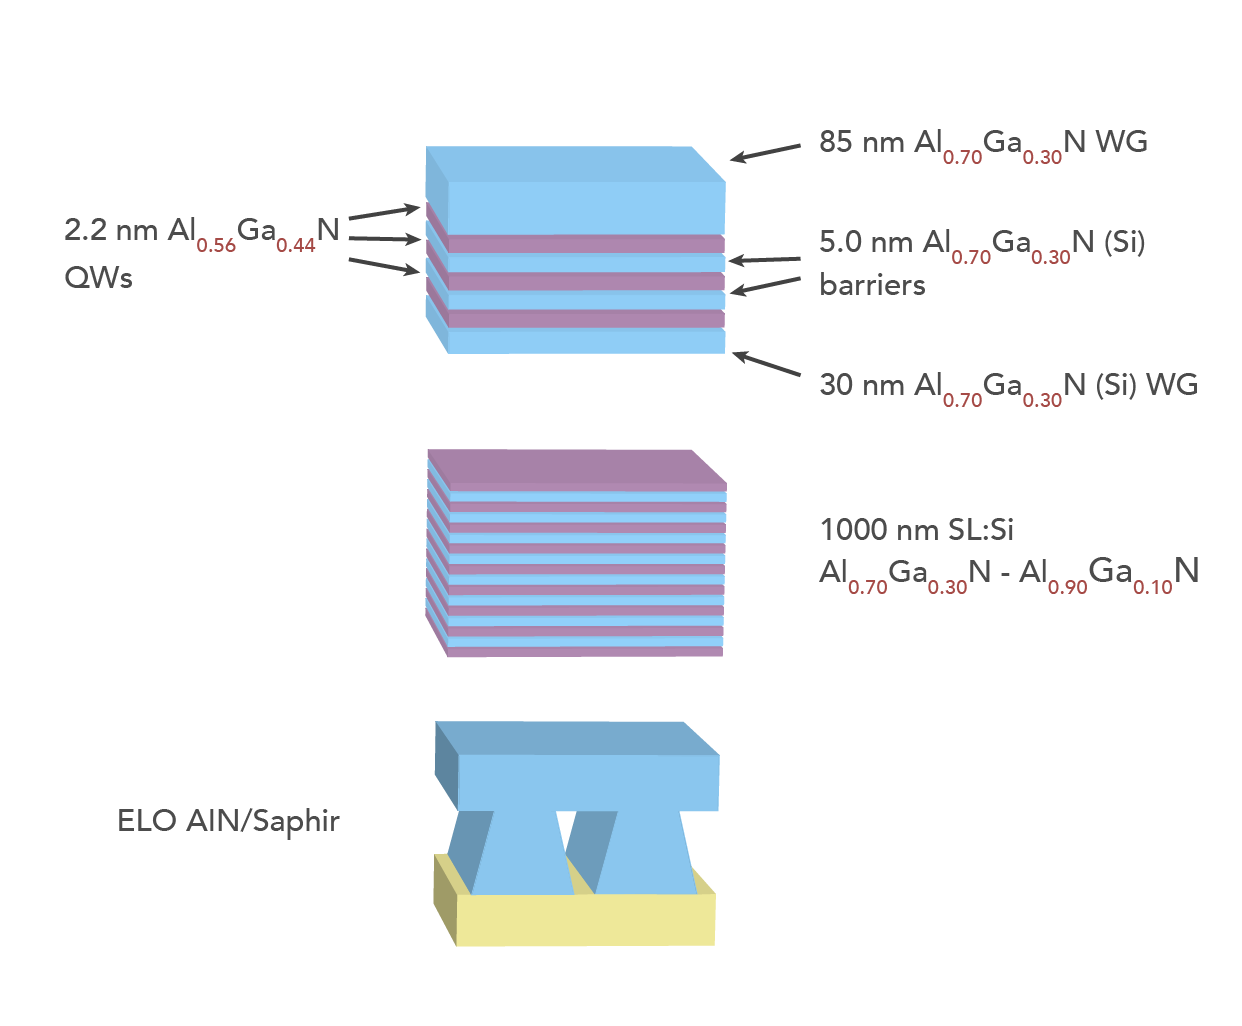
\includegraphics[width=\linewidth]{Bilder/TS4048/ts4048.png}
\caption{Schichtstruktur der untersuchten Proben.}
\label{fig:schichtenelo}
\end{figure}
\noindent 
\vspace{1cm}
%
Stichpunkte. Übergitter nicht wegen Defekten sondern wegen Oberfläche. Glatte Oberfläche wichtig bei Lasern 
%
\begin{figure}[htb]
  \centering
  \begin{minipage}[t]{0.4\textwidth}
    \centering
    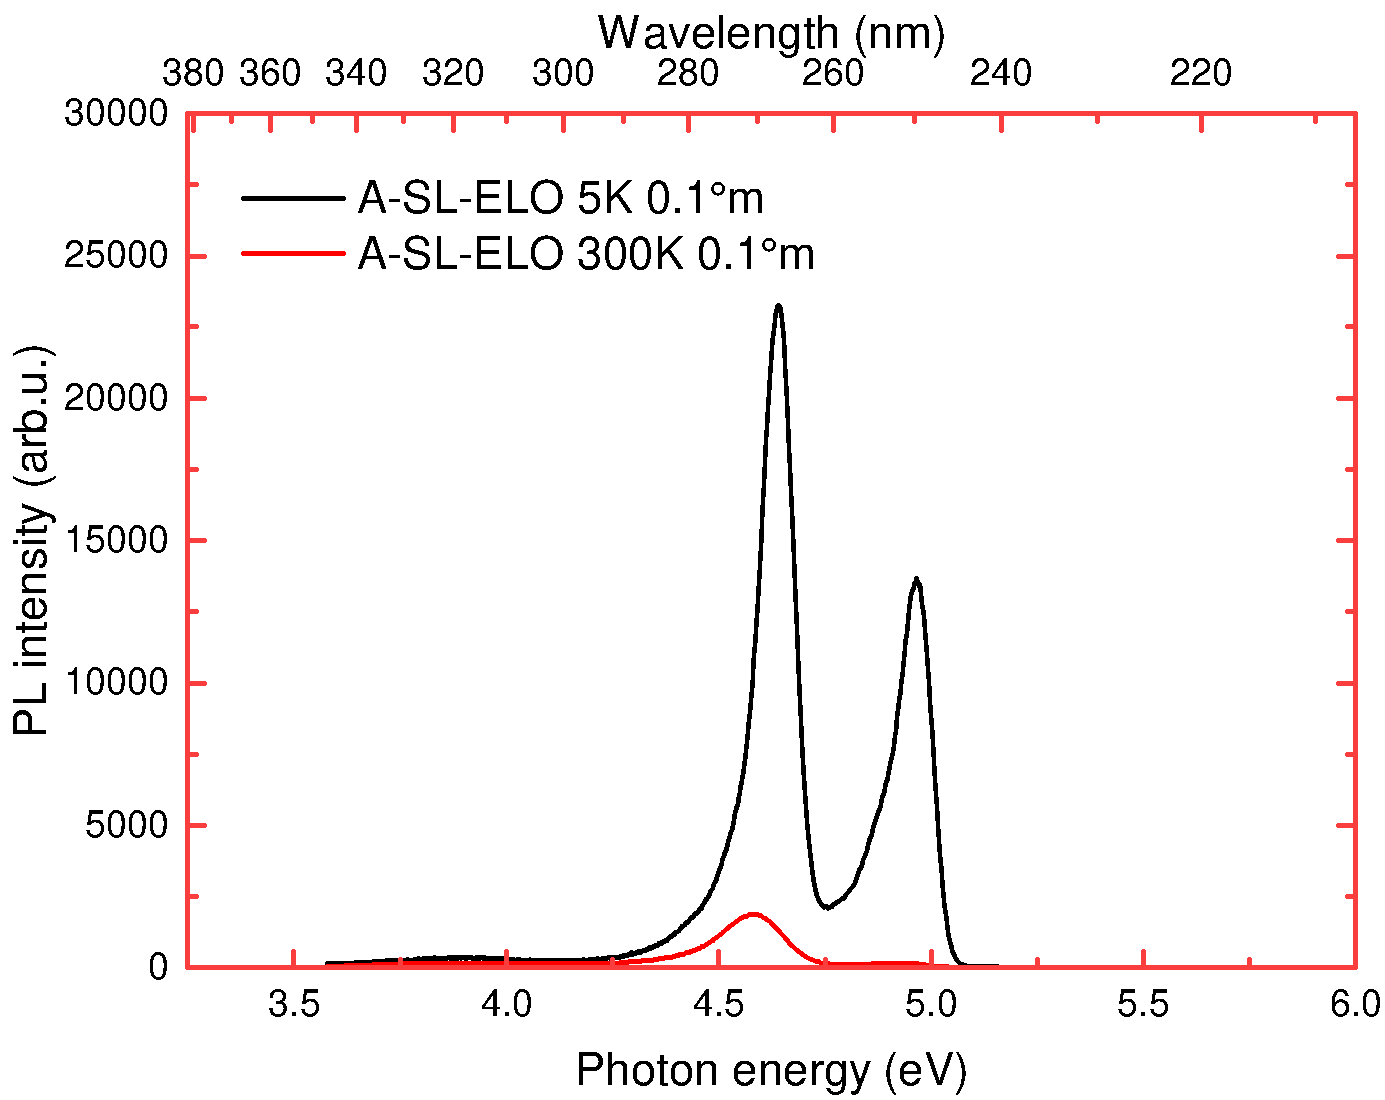
\includegraphics[width=\textwidth]{Bilder/TS4048/aslelo.pdf}
  \end{minipage}
	\hfill
  \begin{minipage}[t]{0.4\textwidth}
    \centering
    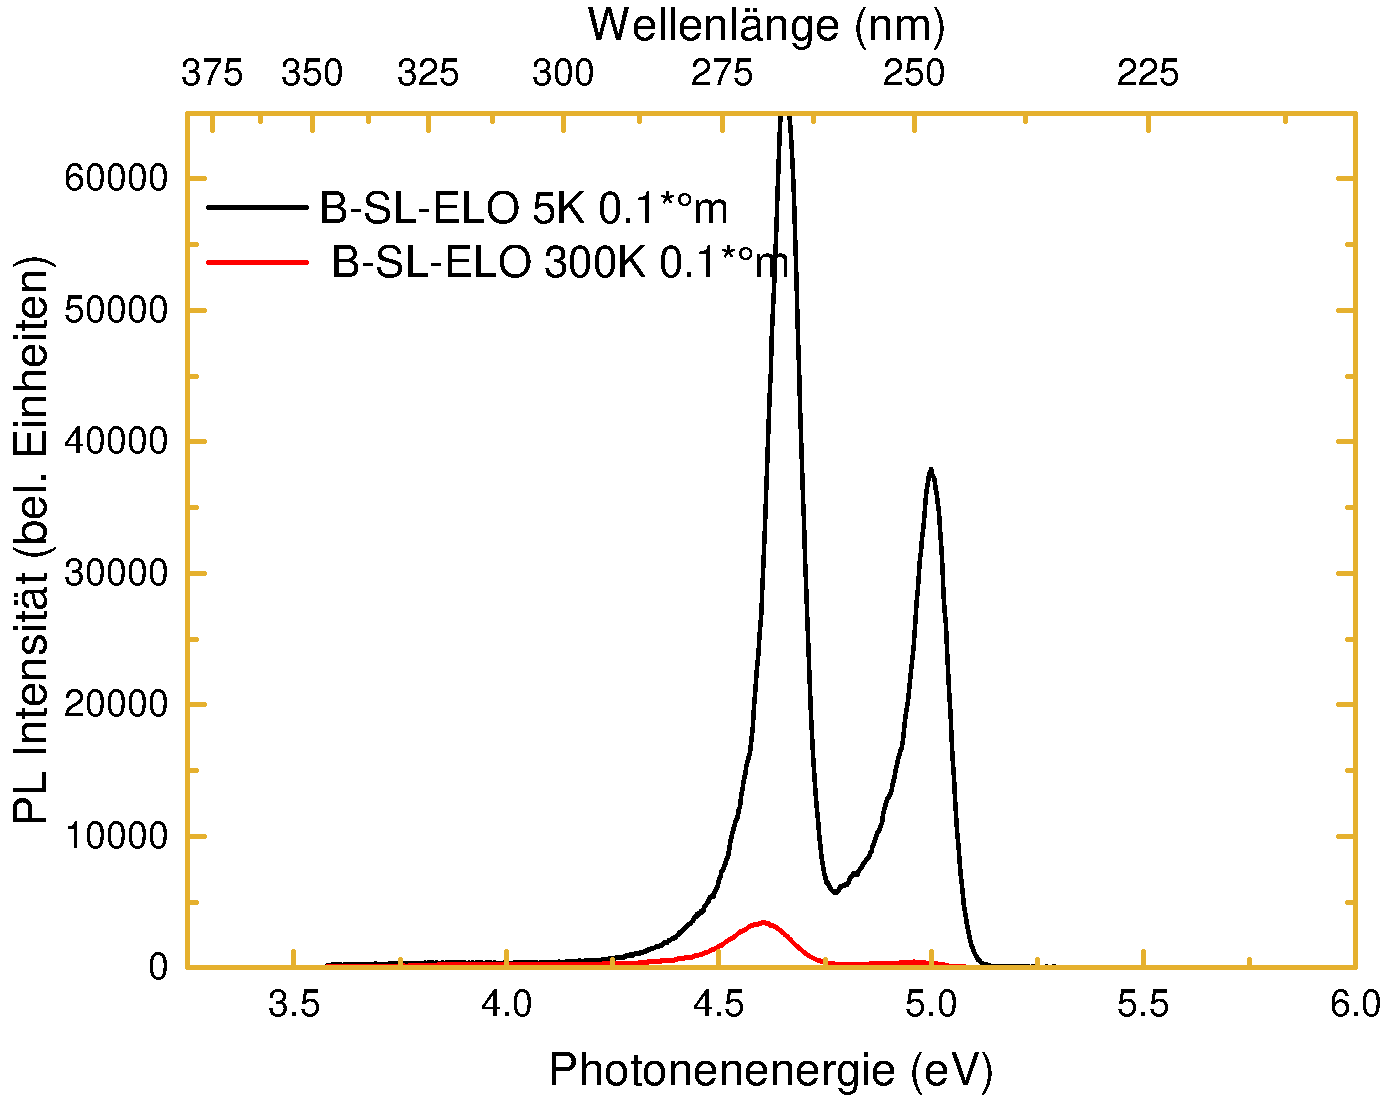
\includegraphics[width=\linewidth]{Bilder/TS4048/bslelo.pdf}
  \end{minipage}
	\hfill
  \begin{minipage}[t]{0.4\textwidth}
    \centering
    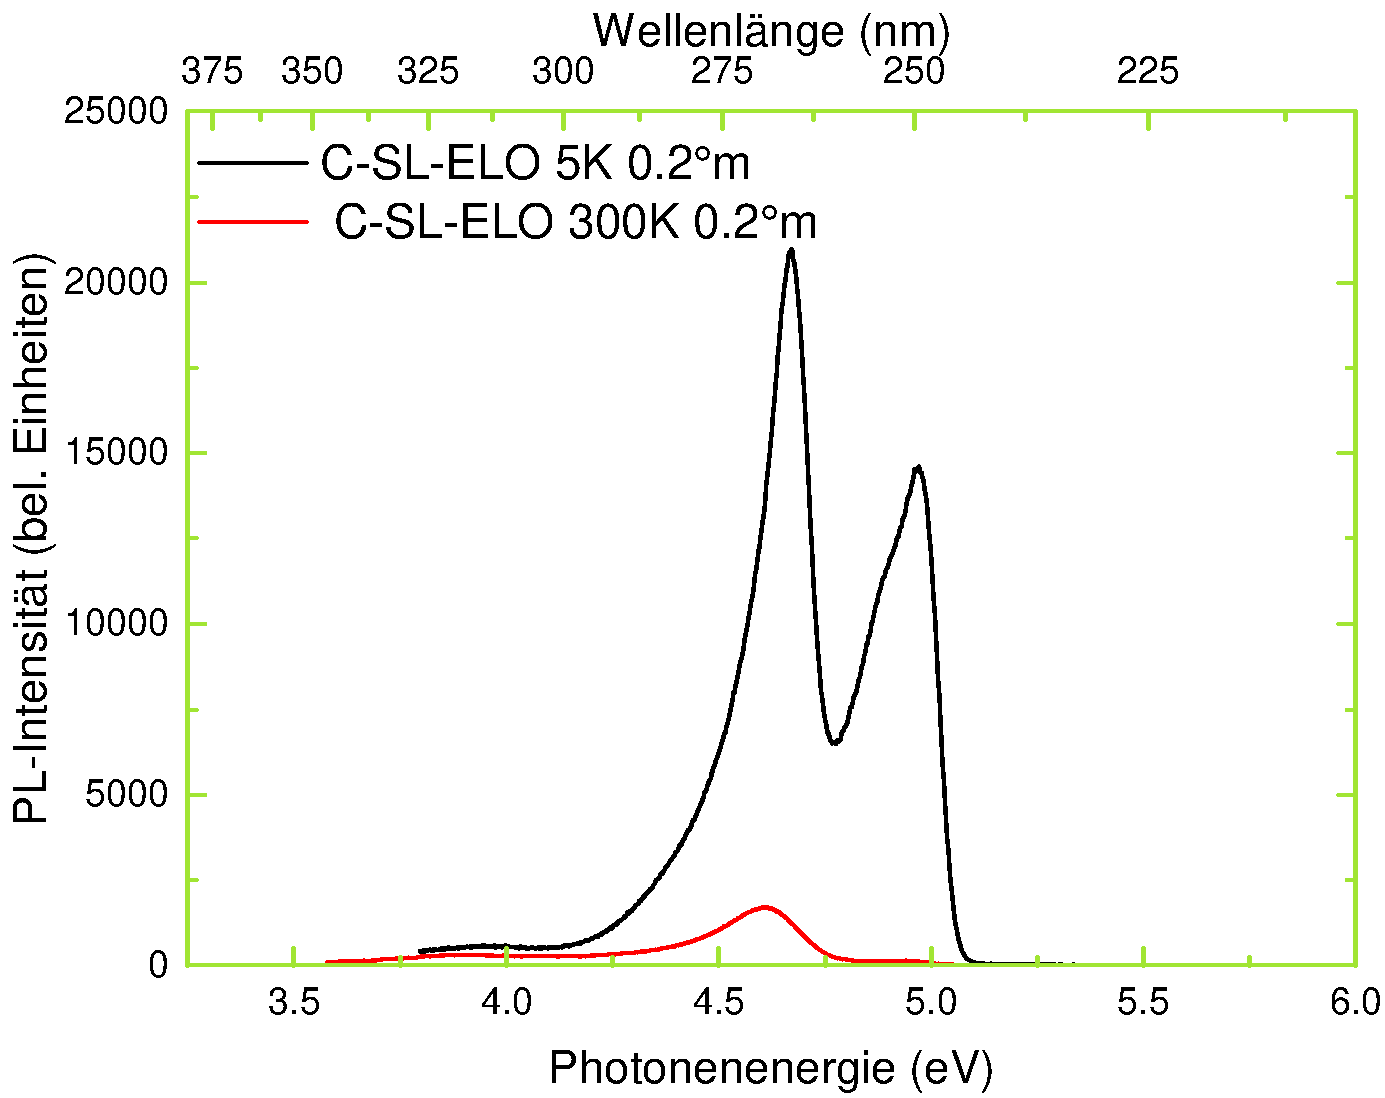
\includegraphics[width=\linewidth]{Bilder/TS4048/cslelo.pdf}
  \end{minipage}
	\caption{Aufnahme der Spektren der Proben A-ELO mit einem Fehlschnittwinkel von $0.1$ in die Standard m-Richtung, Probe B-ELO mit einem Fehlschnittwinkel von $0.1$ die andere m-Richtung und Probe C-ELO mit einem Fehlschnittwinkel von $0.2$ in die standard m-Richtung. }
	\label{fig:spectrassl}
\end{figure}
\noindent 
%
%
\begin{figure}[htb]
  \centering
  \begin{minipage}[t]{0.49\textwidth}
    \centering
    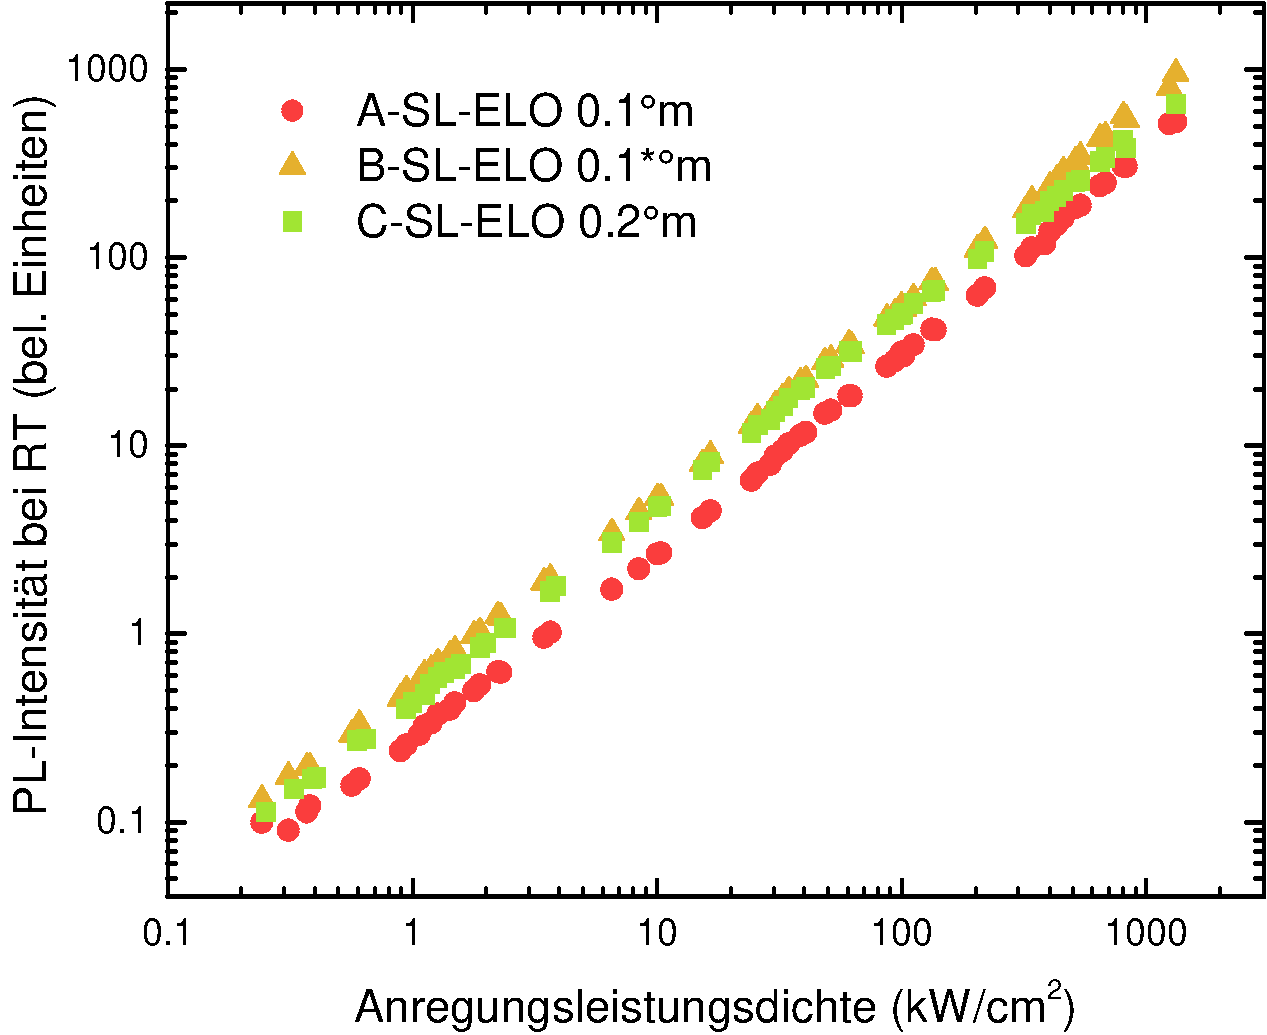
\includegraphics[width=\textwidth]{Bilder/TS4048/intRT.pdf}
		\caption{}
    \label{fig:eloINTrt}
  \end{minipage}
	\hfill
  \begin{minipage}[t]{0.49\textwidth}
    \centering
    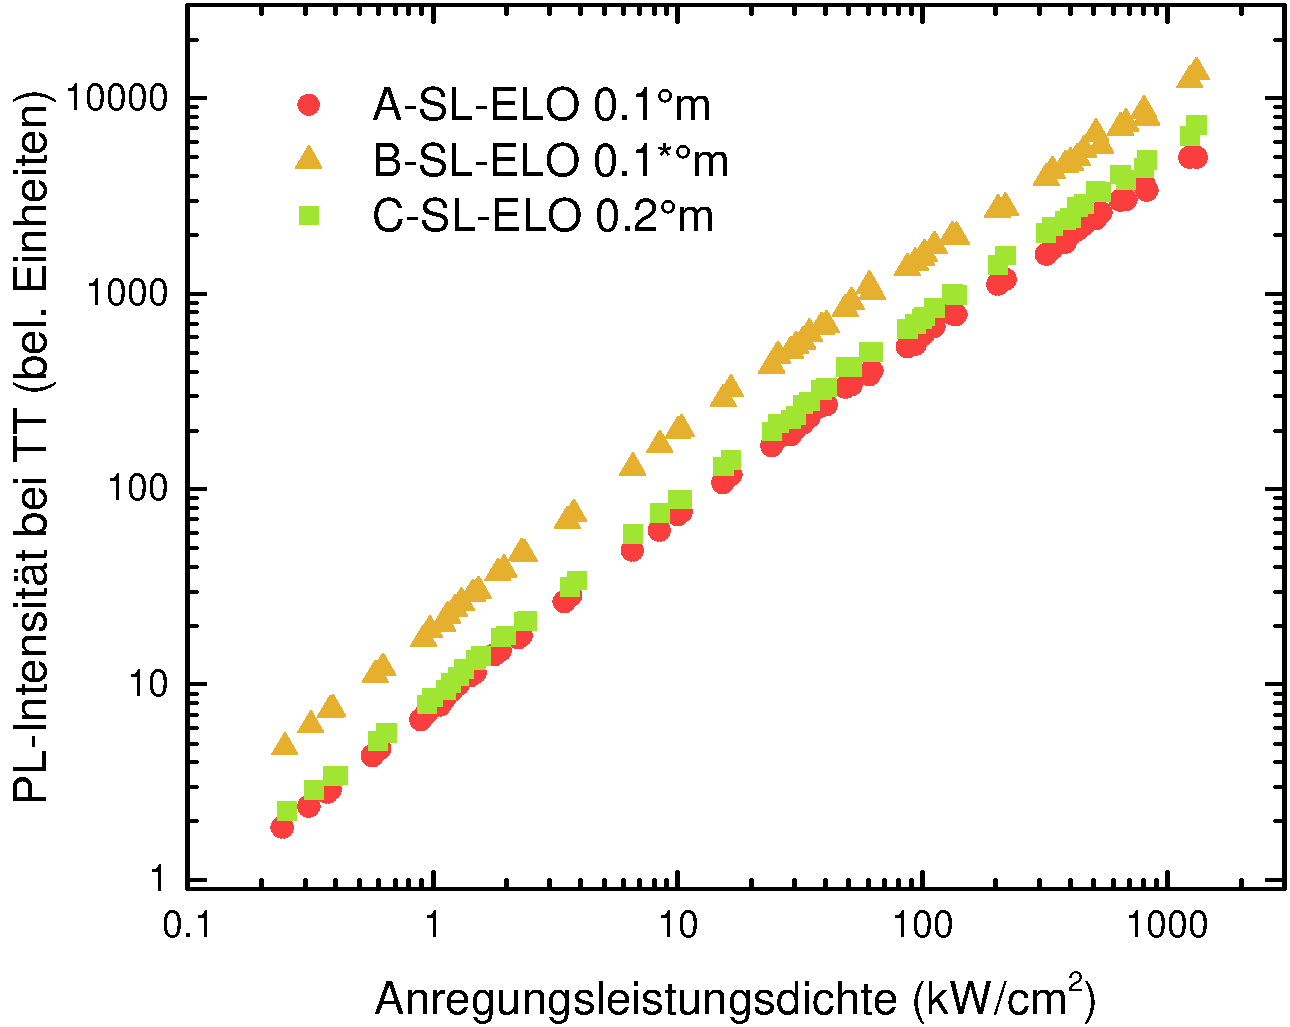
\includegraphics[width=\linewidth]{Bilder/TS4048/intTT.pdf}
    \label{fig:sleloINTtt}
		\caption{}
  \end{minipage}
	\caption{Die integrierte Intensität in Abhängigkeit der Anregungsleistungsdichte bei Raum- und Tieftemperatur in doppelt-logarithmischer Darstellung. }
\end{figure}
\noindent 
% 
%
\begin{figure}[htb]
  \centering
  \begin{minipage}[t]{0.49\textwidth}
    \centering
    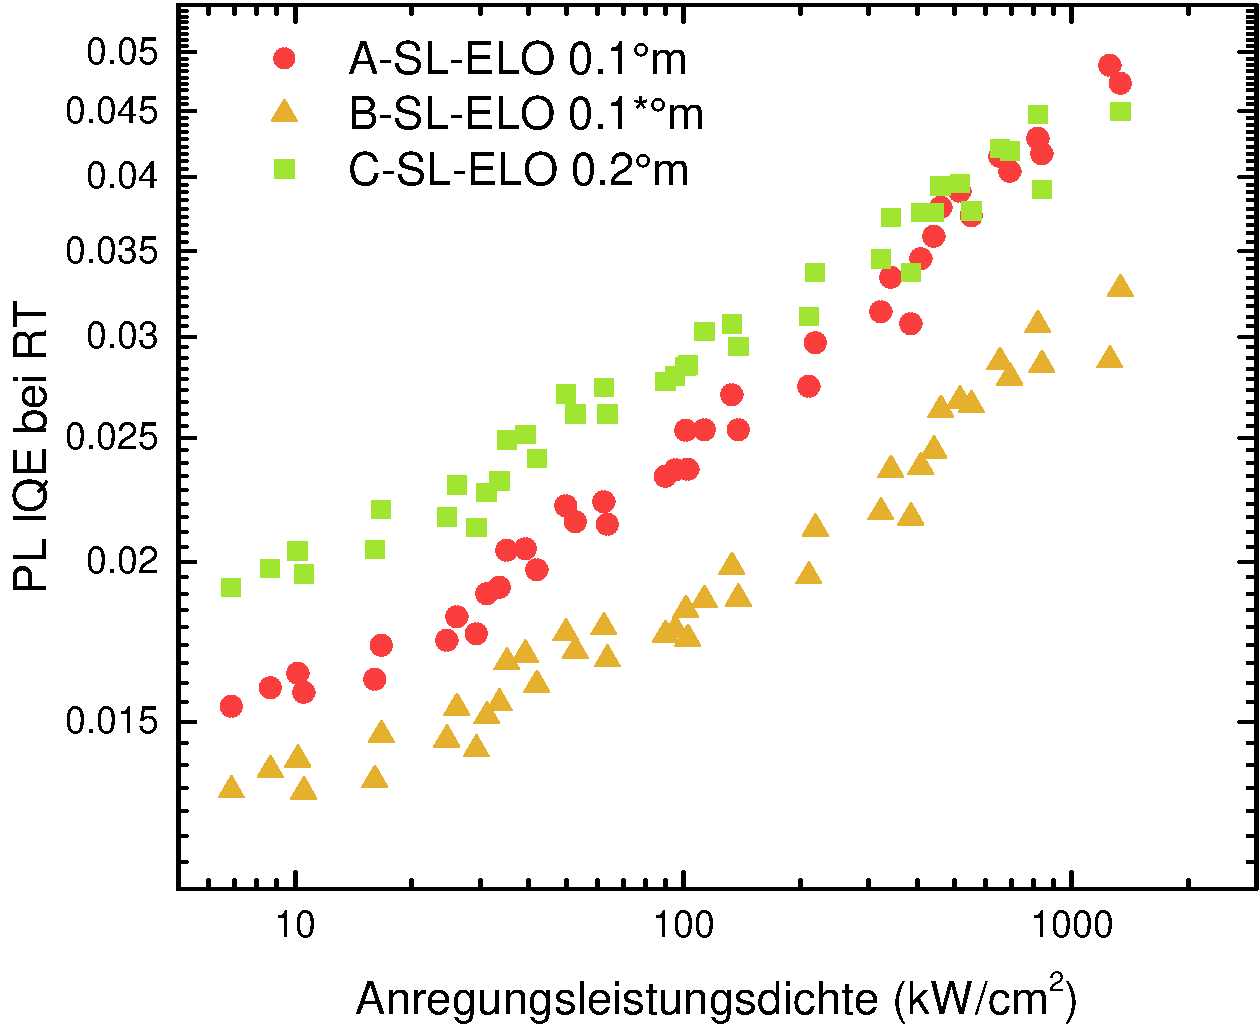
\includegraphics[width=\textwidth]{Bilder/TS4048/corrIQERT.pdf}
    \label{fig:eloiqeRT}
  \end{minipage}
	\hfill
  \begin{minipage}[t]{0.49\textwidth}
    \centering
    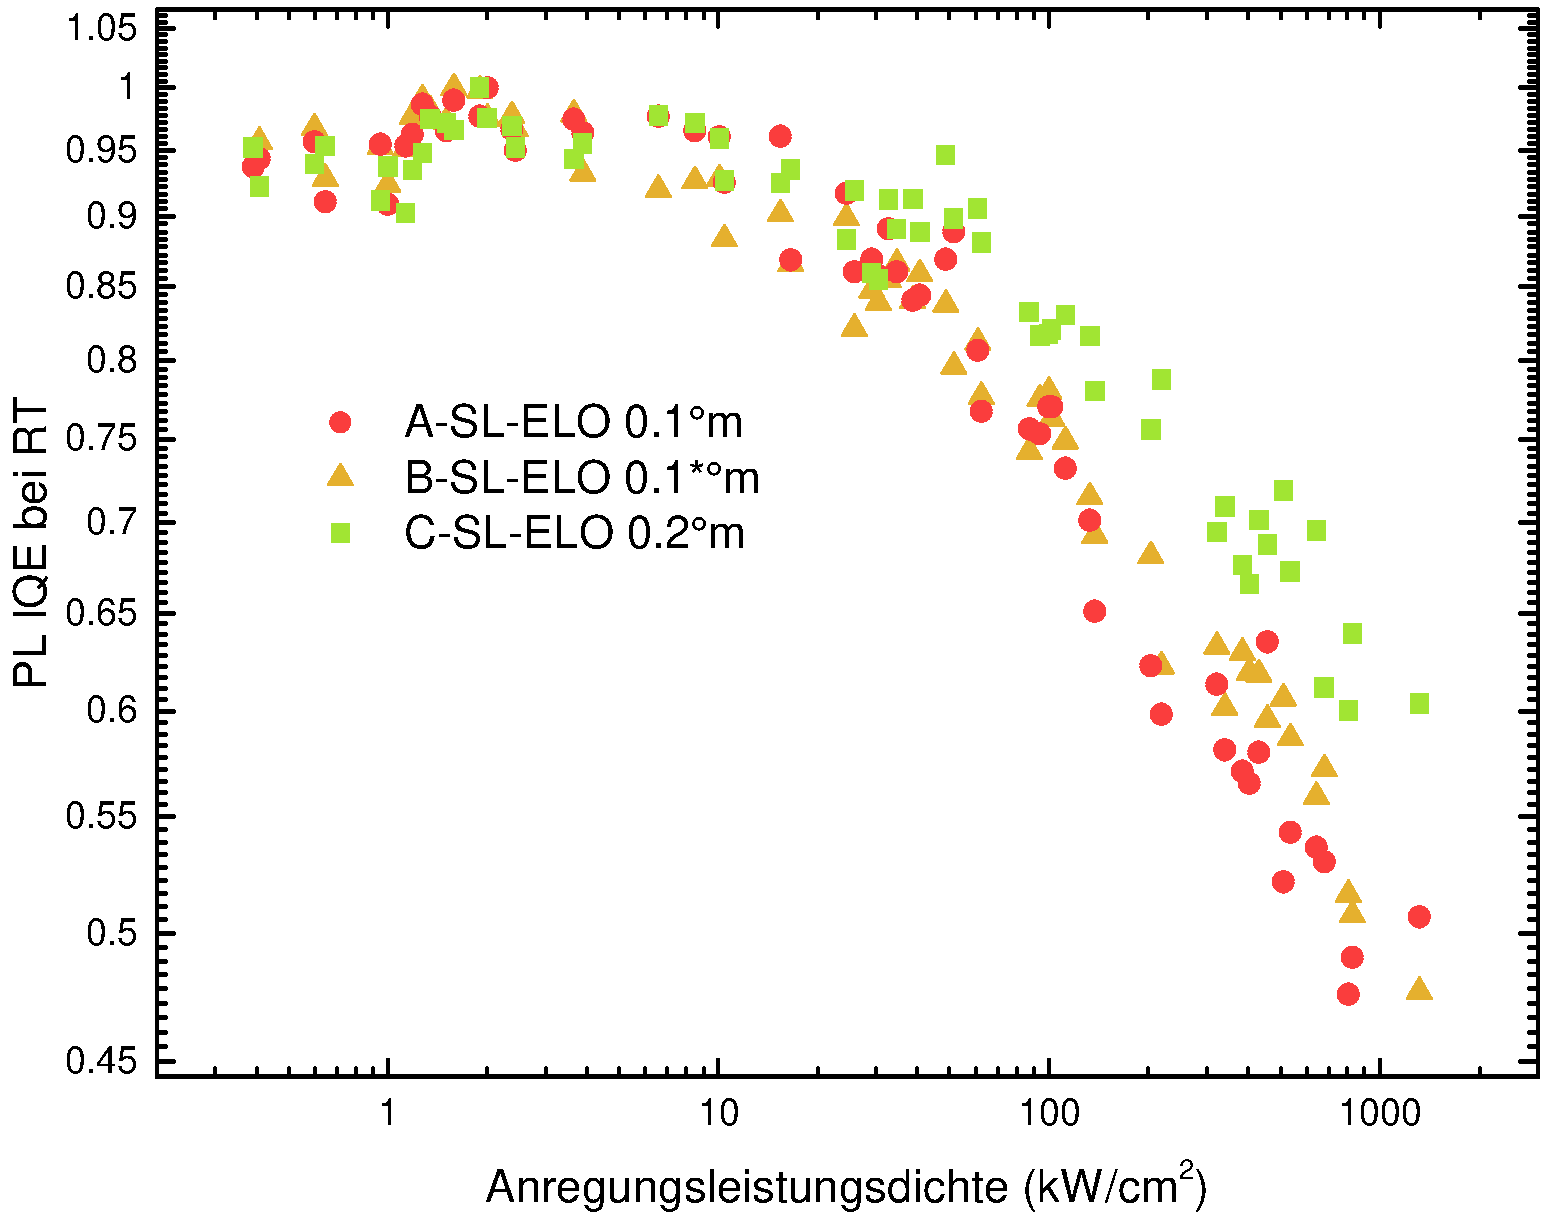
\includegraphics[width=\linewidth]{Bilder/TS4048/IQETT.pdf}
    \label{fig:slelocorriqeRT}
  \end{minipage}
	\caption{Die IQEs für die Proben A-SL-ELO, B-SL-ELO und C-SL-ELO bei Raumtemperatur und Tieftemperatur.}
\end{figure}
\noindent 
%
sadsadsad
%
\begin{figure}[htb]
\begin{tabular}{ccc}
  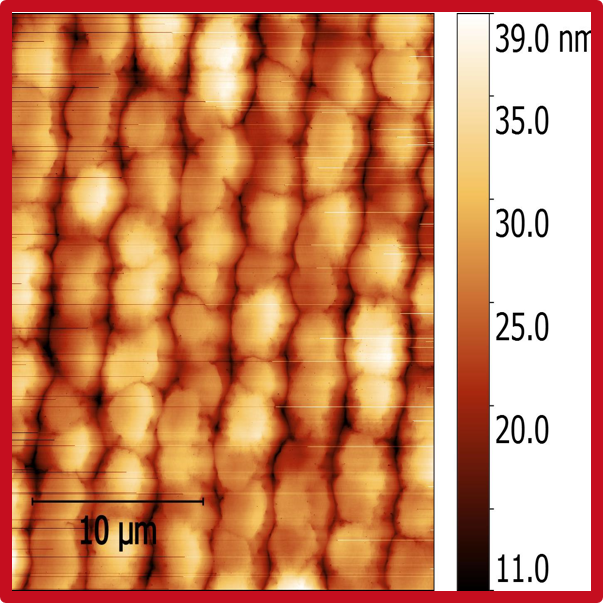
\includegraphics[width=0.35\textwidth]{Bilder/TS4048/aSLELOafm.png} & 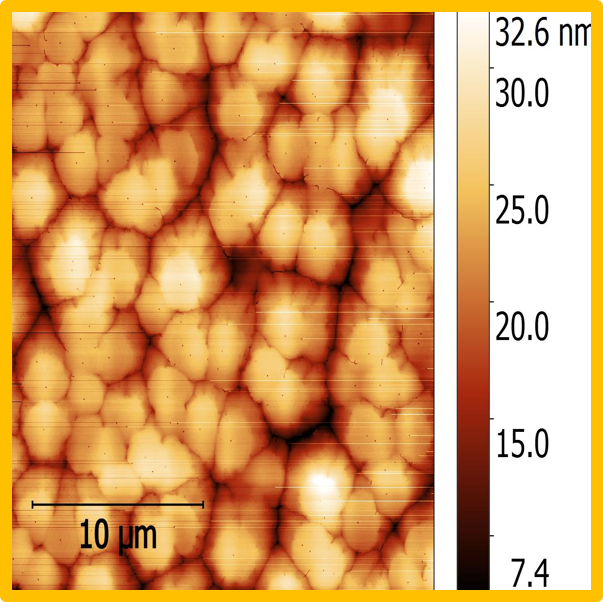
\includegraphics[width=0.35\textwidth]{Bilder/TS4048/bSLELOafm.png}  & 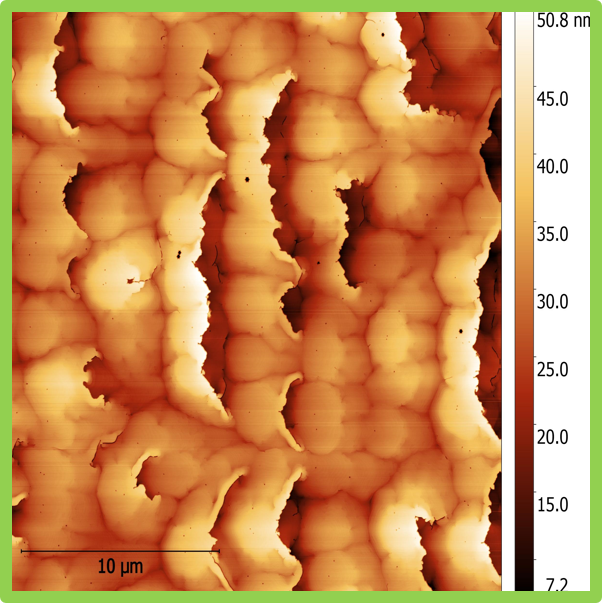
\includegraphics[width=0.35\textwidth]{Bilder/TS4048/cSLELOafm.png} \\
(a) & (b) & (c) \\[6pt]
 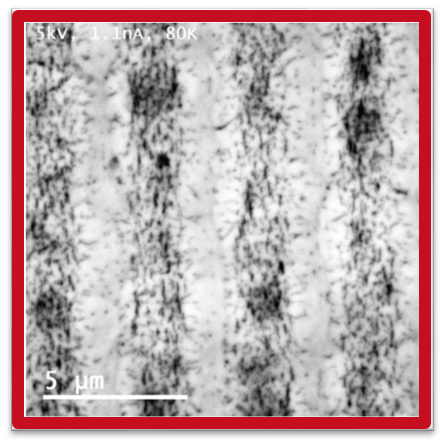
\includegraphics[width=0.35\textwidth]{Bilder/TS4048/aSLELOcl2.png} &   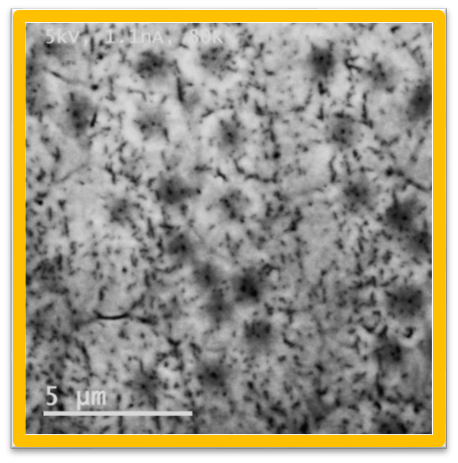
\includegraphics[width=0.35\textwidth]{Bilder/TS4048/bSLELOcl2.png} & 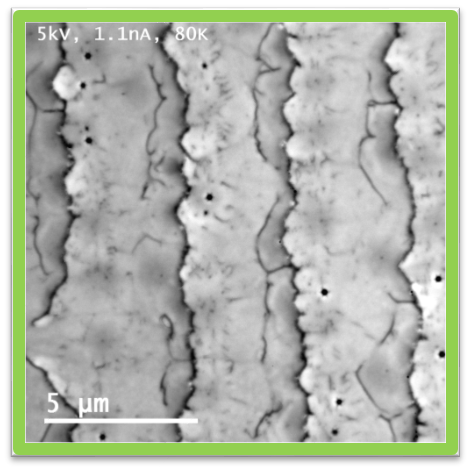
\includegraphics[width=0.35\textwidth]{Bilder/TS4048/cSLELOcl2.png}  \\
(c)  & (d) & (e)   \\[6pt]
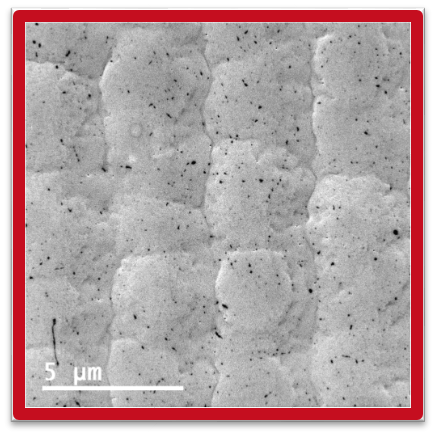
\includegraphics[width=0.35\textwidth]{Bilder/TS4048/aSLELOcl1.png} & 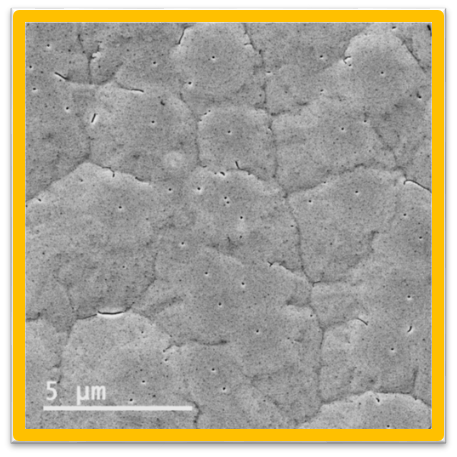
\includegraphics[width=0.35\textwidth]{Bilder/TS4048/bSLELOcl1.png}  & 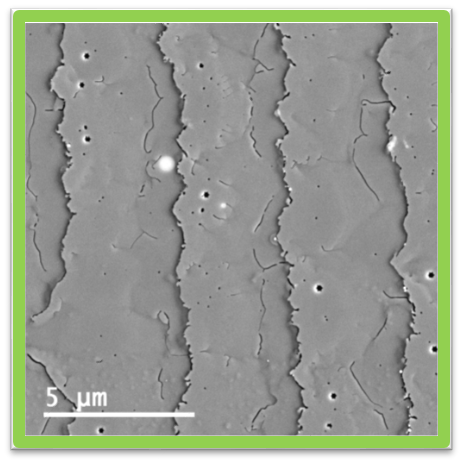
\includegraphics[width=0.35\textwidth]{Bilder/TS4048/cSLELOcl1.png} \\
(f)  & (g) & (h)   \\[6pt]
\end{tabular}
\caption{AFM-Bilder (a, b) und eine Limi-Aufnahme (c) von Christian Kuhn aufgenommen. SEM (c, d, e) und panchromatische CL-Aufnahmen(f, g, h) an den selben Stellen gemessen von Ute Zeimer (FBH)}
\label{fig:morph1}
\end{figure}
\noindent 
sadsadsadsa